% ===========================================================================
%  Rapport de projet – Deep Learning for Computer Vision 2025/2026
%  Détection de bâtiments sur imagerie satellitaire avec YOLOv5
% ===========================================================================
\documentclass[12pt,a4paper]{article}

% ---- Encodage et langue ----
\usepackage[utf8]{inputenc}
\usepackage[T1]{fontenc}
\usepackage[french]{babel}

% ---- Mise en page ----
\usepackage[margin=2.5cm]{geometry}
\usepackage{setspace}
\onehalfspacing

% ---- Typographie et math ----
\usepackage{amsmath,amssymb}
\usepackage{lmodern}

% ---- Couleurs (nécessaire pour la syntaxe de mélange blue!70!black) ----
\usepackage{xcolor}

% ---- Figures et tableaux ----
\usepackage{graphicx}
\usepackage{float}
\usepackage{booktabs}
\usepackage{array}
\usepackage{tabularx}
\usepackage{multirow}

% ---- Code source ----
\usepackage{listings}
\lstset{
  basicstyle=\ttfamily\small,
  breaklines=true,
  frame=single,
  language=Python,
  keywordstyle=\bfseries\color{blue!70!black},
  commentstyle=\itshape\color{green!50!black},
  stringstyle=\color{red!60!black},
  numbers=left,
  numberstyle=\tiny\color{gray},
  showstringspaces=false,
}

% ---- Liens et références ----
\usepackage[colorlinks=true,linkcolor=blue!60!black,citecolor=blue!60!black,urlcolor=blue!60!black]{hyperref}

% ---- En-tête ----
\usepackage{fancyhdr}
\pagestyle{fancy}
\fancyhf{}
\fancyhead[L]{\small Détection de bâtiments -- YOLOv5}
\fancyhead[R]{\small Master SISE 2025--2026}
\fancyfoot[C]{\thepage}

\graphicspath{{figures/}}

% =====================================================================
\begin{document}

% ---- Page de titre ----
\begin{titlepage}
\centering
\vspace*{2cm}

{\LARGE\bfseries Détection de bâtiments sur imagerie satellitaire\\[0.3em]
avec YOLOv5 Nano}

\vspace{1.5cm}
{\Large Deep Learning for Computer Vision\\[0.2em]
Projet 2025/2026}

\vspace{1.5cm}
{\large
\textbf{Olivier BOROT} \\[0.3em]
\textbf{Marin NAGY}
}

\vspace{1.5cm}
{\large
Université Lumière Lyon~2 --- Master SISE
}

\vspace{1cm}
{\large Mars 2026}

\vfill
\end{titlepage}

% ---- Table des matières ----
\tableofcontents
\newpage

% =====================================================================
\section{Introduction}
% =====================================================================

L'identification automatique de types de bâtiments à partir d'images satellitaires constitue un enjeu majeur pour l'aménagement du territoire, la cartographie et la surveillance environnementale. Ce projet propose une approche basée sur le \emph{deep learning} pour détecter et classifier six catégories de structures à partir de vues aériennes haute résolution.

Nous utilisons l'architecture \textbf{YOLOv5 Nano} (\texttt{yolov5n}), un réseau de détection d'objets en temps réel, que nous adaptons par \emph{transfer learning} à notre jeu de données personnalisé composé d'images satellitaires Mapbox annotées à l'aide de données OpenStreetMap (OSM) et de l'outil Roboflow.

Le présent rapport décrit successivement : la construction du jeu de données (section~\ref{sec:dataset}), l'architecture du modèle (section~\ref{sec:architecture}), le protocole d'entraînement (section~\ref{sec:training}), les résultats quantitatifs et qualitatifs (section~\ref{sec:results}), et une discussion finale (section~\ref{sec:discussion}).

% =====================================================================
\section{Jeu de données}\label{sec:dataset}
% =====================================================================

\subsection{Collecte des images satellitaires}

La collecte de données repose sur un pipeline automatisé développé en Python (voir notebook \texttt{01 - Pipeline\_complète.ipynb}). Les étapes clés sont les suivantes :

\begin{enumerate}
    \item \textbf{Sélection des zones d'intérêt.}
    Nous avons sélectionné les 20 villes les plus peuplées de France ainsi que 100 coordonnées rurales réparties aléatoirement sur le territoire français.
    Pour chaque ville, une \emph{bounding box} de 10\,km $\times$ 10\,km est définie autour du centre, puis 10 points aléatoires sont échantillonnés dans cette zone.
    Au total, cela donne environ 300 points de collecte ($20 \times 10 + 100$).

    \item \textbf{Téléchargement des images.}
    Pour chaque coordonnée, une \emph{bounding box} précise est calculée à l'aide d'une projection Lambert~93 (EPSG:2154) avec une résolution de 0,4\,m/pixel et une taille d'image de $512 \times 542$\,pixels ($512 + 30$\,px de filigrane Mapbox). L'image satellitaire correspondante est récupérée via l'API \emph{Mapbox Static Images} (style \texttt{satellite-v9}).

    \item \textbf{Recadrage.}
    Le filigrane Mapbox (30\,pixels du bas) est supprimé, produisant des images utiles de $512 \times 512$\,pixels.
\end{enumerate}

\subsection{Annotation automatique via OpenStreetMap}

Plutôt que d'annoter manuellement chaque image, nous exploitons les données bâtimentaires d'OpenStreetMap à l'aide de la bibliothèque \texttt{osmnx} :

\begin{enumerate}
    \item Les polygones de bâtiments situés dans la \emph{bounding box} de chaque image sont récupérés avec \texttt{ox.features\_from\_bbox(tags=\{"building": True\})}.
    \item Un dictionnaire de correspondance (\texttt{osm\_to\_category\_mapping.json}) associe les tags OSM (\texttt{house}, \texttt{apartments}, etc.) à nos six classes.
    \item Les polygones complexes sont convertis en \emph{bounding boxes} rectangulaires via \texttt{.envelope}.
    \item Un algorithme de nettoyage itératif fusionne les \emph{bounding boxes} qui se chevauchent au-delà d'un seuil de 30\,\% (module \texttt{clean\_overlapping\_bboxes}).
    \item Les annotations résultantes sont converties au format YOLO (\texttt{class\_id x\_center y\_center width height}, coordonnées normalisées) par le module \texttt{format\_yolo\_labels}.
\end{enumerate}

\subsection{Finalisation avec Roboflow}

Le jeu de données a ensuite été importé dans \textbf{Roboflow} pour :
\begin{itemize}
    \item vérifier et corriger manuellement les annotations ;
    \item redimensionner les images à $640 \times 640$\,pixels (étirement) ;
    \item appliquer une auto-orientation (strip EXIF).
\end{itemize}

\noindent\textbf{Remarque :} l'intégralité des 144 images a été exportée en un seul dossier depuis Roboflow. Cependant, un découpage rigoureux a été implémenté dans le notebook d'entraînement (\texttt{Final\_01\_Training.ipynb}) :
\begin{itemize}
    \item \textbf{80\,\%} pour l'entraînement ($\sim$115 images) ;
    \item \textbf{10\,\%} pour la validation pendant l'entraînement ($\sim$14 images) ;
    \item \textbf{10\,\%} pour le test final, isolés dès le début et jamais vus par le modèle ($\sim$15 images).
\end{itemize}

\subsection{Statistiques du jeu de données}

\begin{table}[H]
\centering
\begin{tabularx}{\linewidth}{>{\raggedright\arraybackslash}X r}
	oprule
	extbf{Caractéristique} & \textbf{Valeur} \\
\midrule
Nombre total d'images & 144 \\
Résolution finale & $640 \times 640$ pixels \\
Format d'annotation & YOLO v5 PyTorch \\
Nombre de classes & 6 \\
Total annotations & 2\\,461 \\
\bottomrule
\end{tabularx}
\caption{Résumé du jeu de données.}
\label{tab:dataset}
\end{table}

La figure~\ref{fig:class_dist} montre la répartition des annotations par classe. On observe un fort déséquilibre : la classe \texttt{maison} domine avec 1\,245 annotations (50,6\,\%), suivie de \texttt{immeuble} (788, 32\,\%). Les classes \texttt{usine} (69) et \texttt{villa} (17) sont très sous-représentées, ce qui constitue un défi pour l'entraînement.

\begin{figure}[H]
\centering
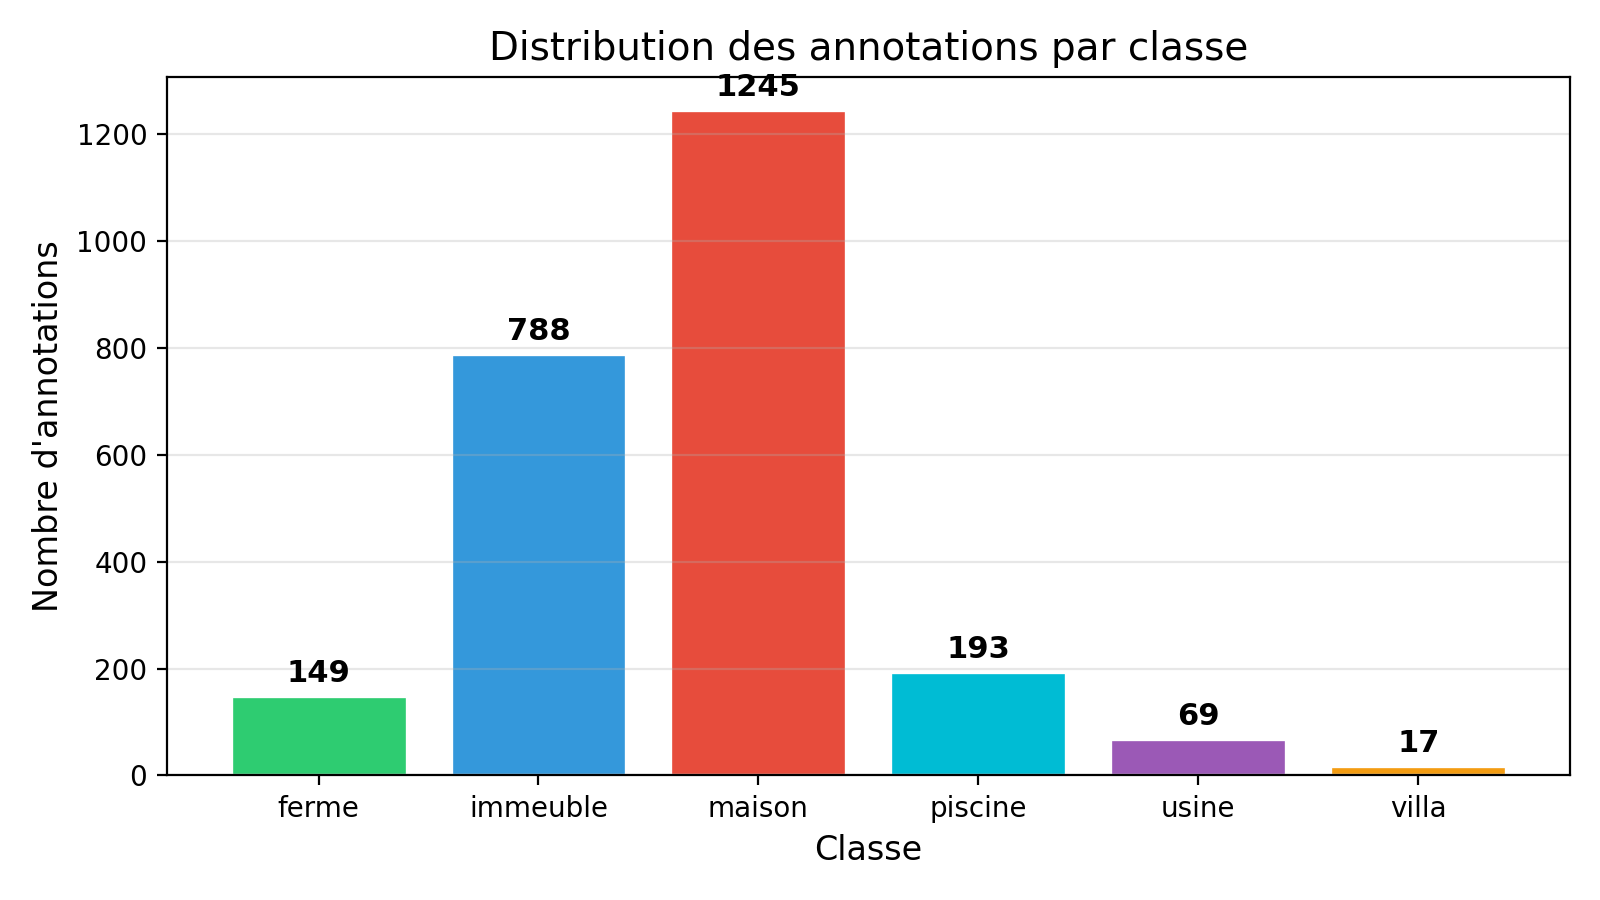
\includegraphics[width=0.85\textwidth]{class_distribution.png}
\caption{Distribution des annotations par classe dans le jeu de données.}
\label{fig:class_dist}
\end{figure}

Les six classes définies sont :

\begin{table}[H]
\centering
\begin{tabularx}{\linewidth}{c >{\raggedright\arraybackslash}X X}
\toprule
\textbf{ID} & \textbf{Classe} & \textbf{Description} \\
\midrule
0 & \texttt{ferme} & Exploitation agricole \\
1 & \texttt{immeuble} & Immeuble résidentiel ou de bureaux \\
2 & \texttt{maison} & Maison individuelle \\
3 & \texttt{piscine} & Piscine \\
4 & \texttt{usine} & Bâtiment industriel \\
5 & \texttt{villa} & Villa / grande maison \\
\bottomrule
\end{tabularx}
\caption{Classes du jeu de données.}
\label{tab:classes}
\end{table}

\subsection{Exemples d'images}

La figure~\ref{fig:samples} présente des exemples d'images du jeu d'entraînement après redimensionnement à $640 \times 640$. La figure~\ref{fig:annotated} montre ces mêmes images avec les \emph{bounding boxes} de vérité terrain superposées.

\begin{figure}[H]
\centering
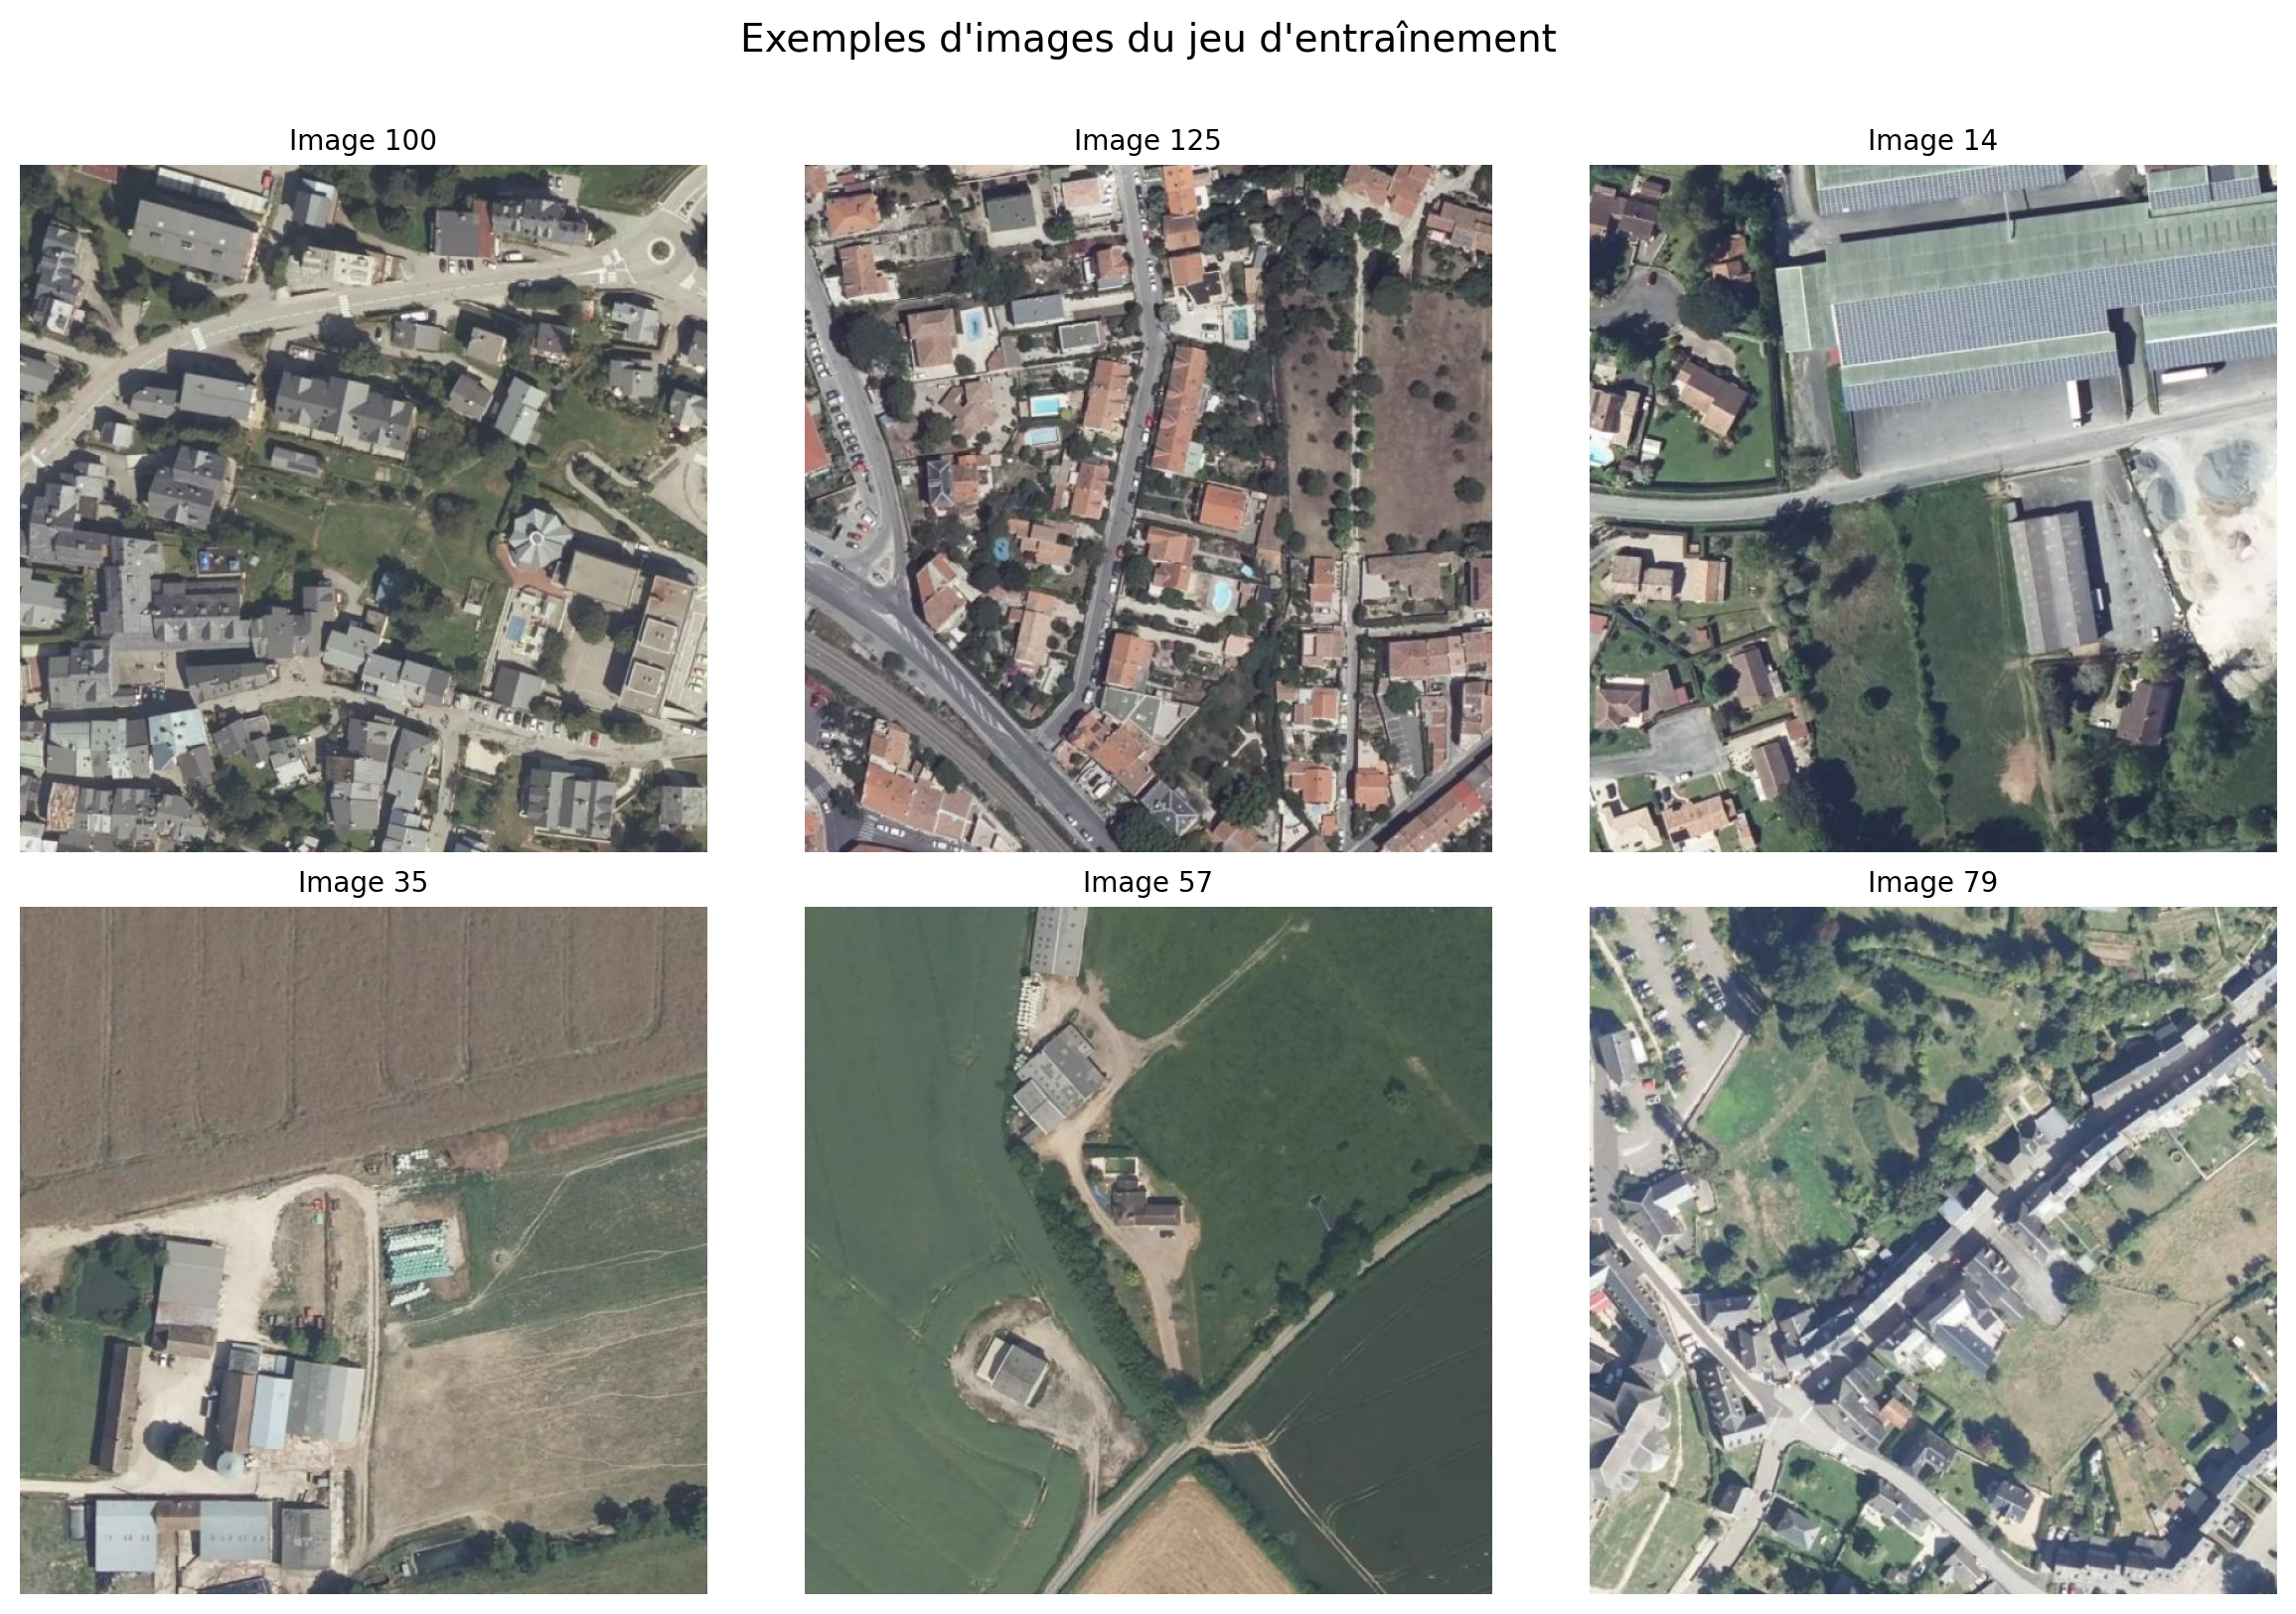
\includegraphics[width=0.95\textwidth]{sample_grid.png}
\caption{Exemples d'images satellitaires du jeu d'entraînement ($640 \times 640$).}
\label{fig:samples}
\end{figure}

\begin{figure}[H]
\centering
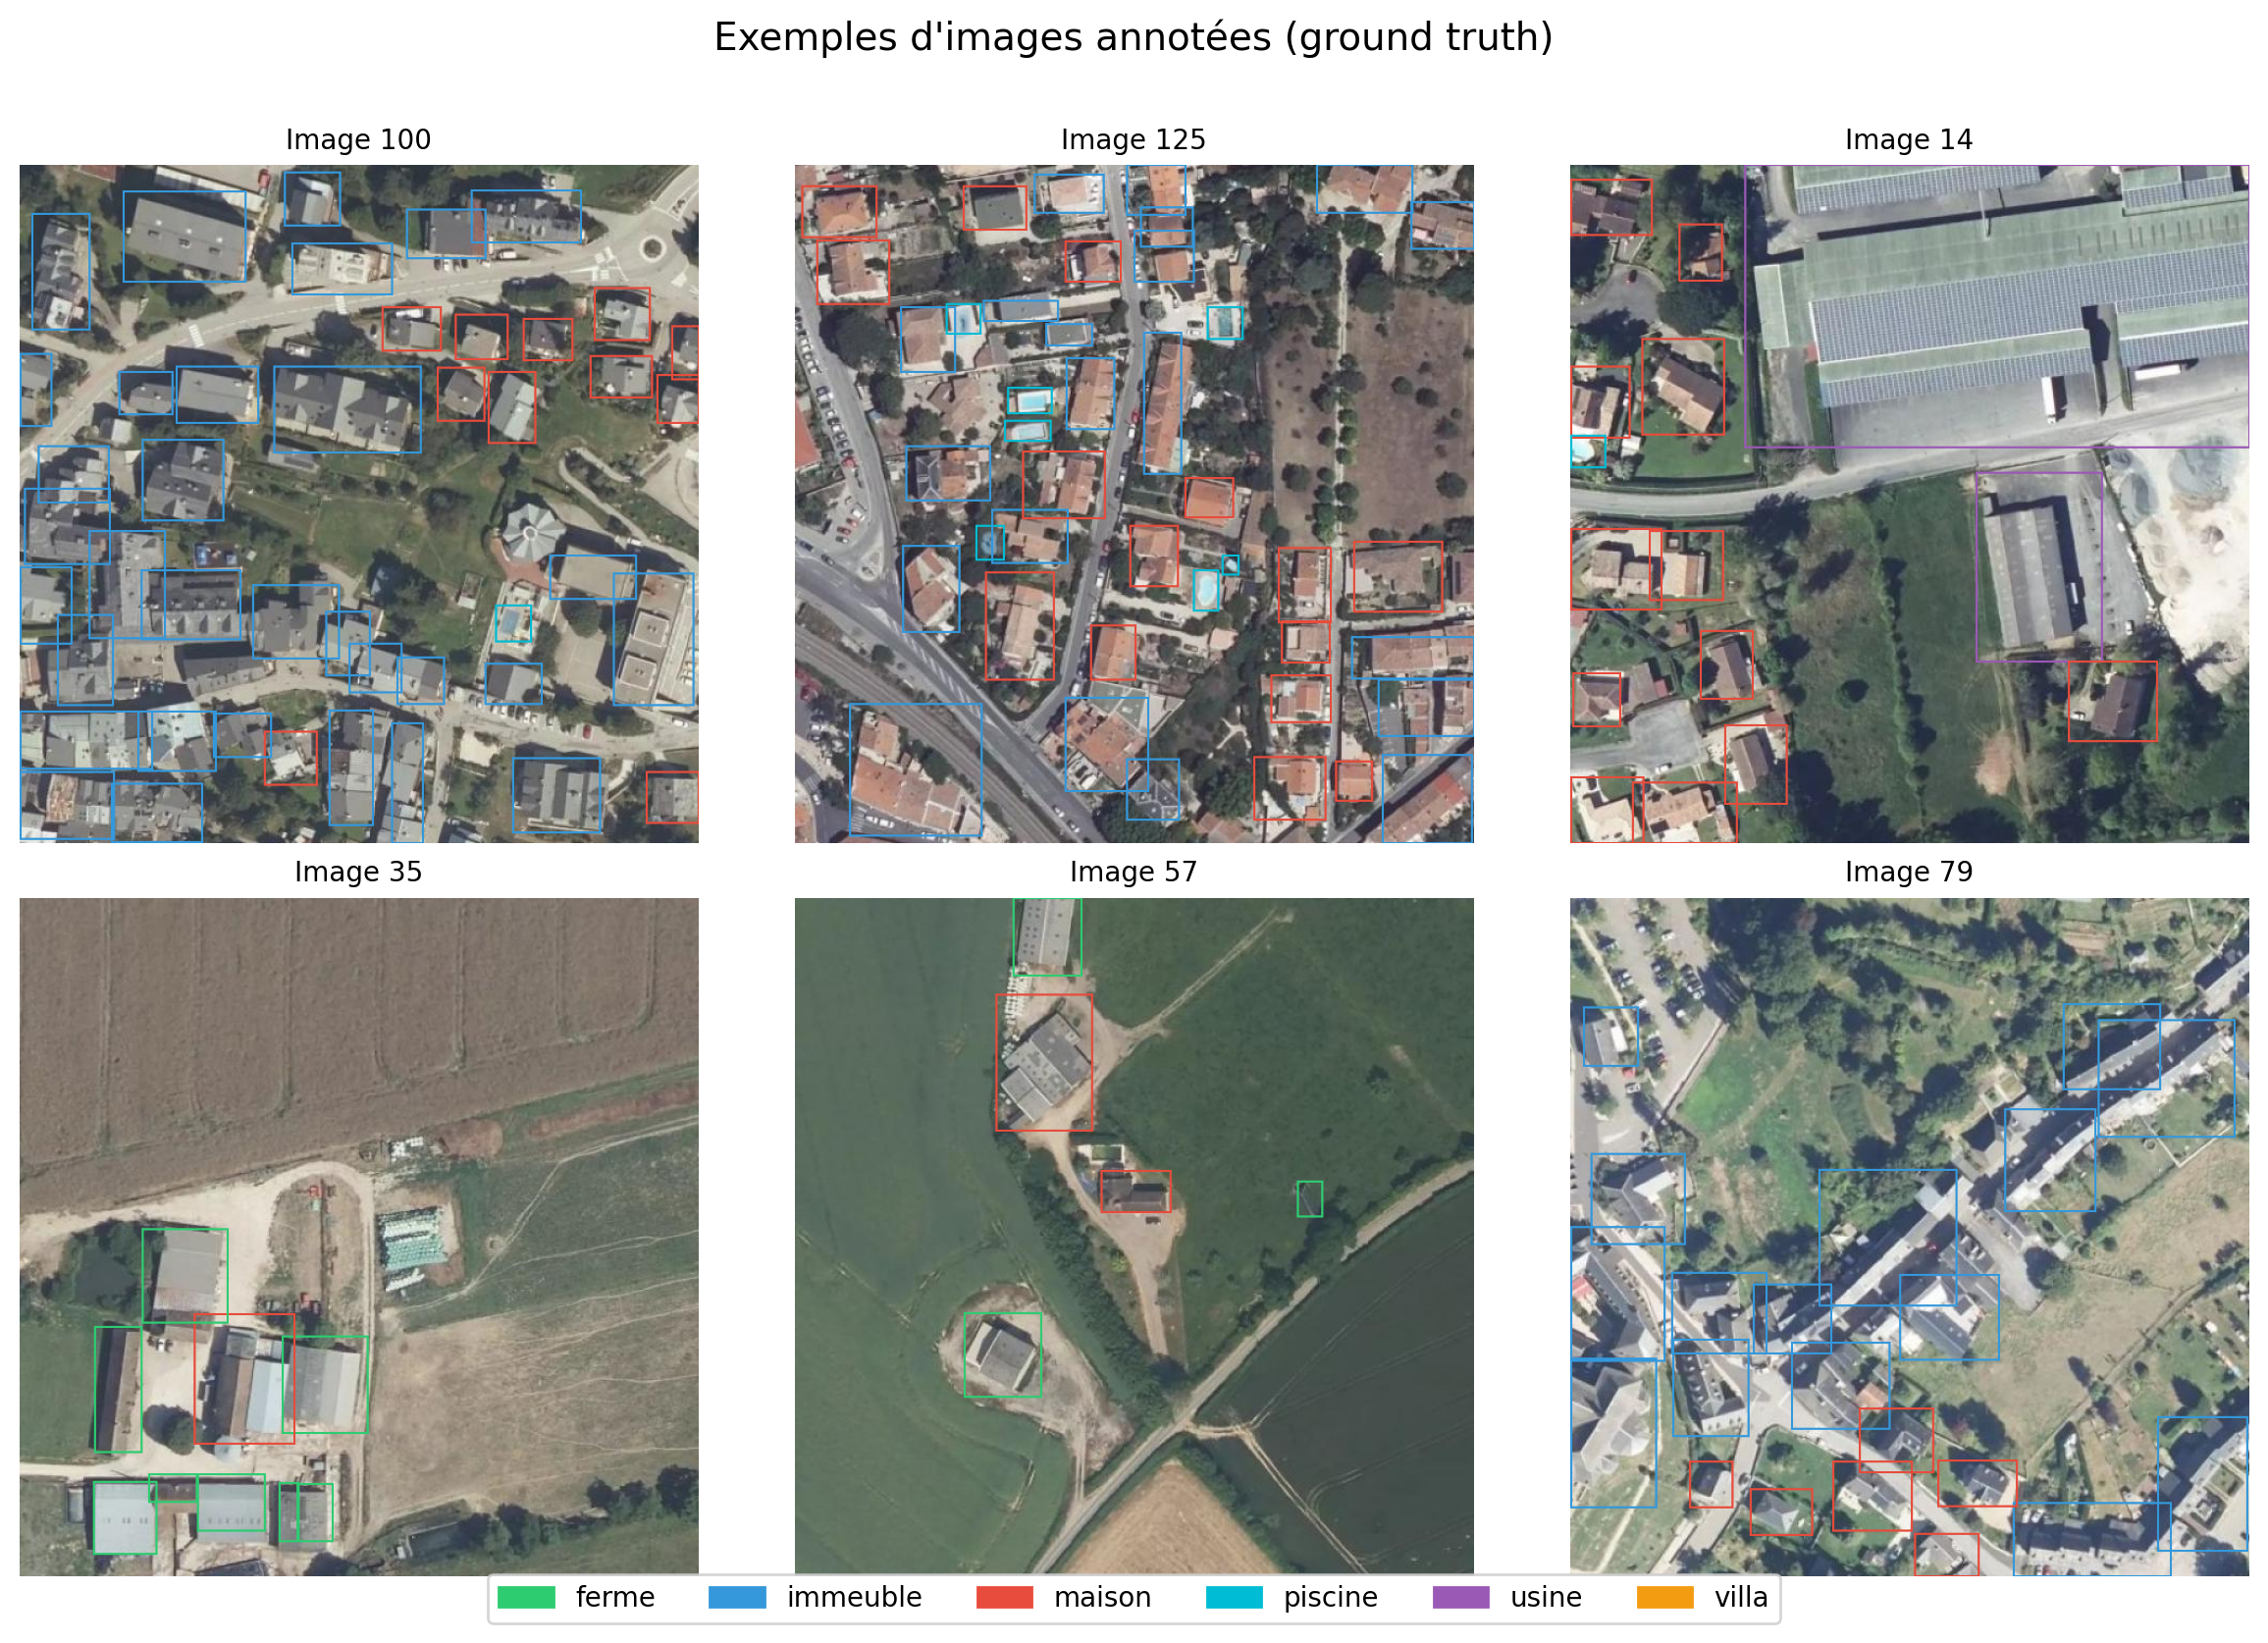
\includegraphics[width=0.95\textwidth]{annotated_grid.png}
\caption{Exemples d'images avec annotations \emph{ground truth} (bounding boxes colorées par classe).}
\label{fig:annotated}
\end{figure}

% =====================================================================
\section{Architecture du modèle}\label{sec:architecture}
% =====================================================================

\subsection{YOLOv5 --- Présentation générale}

YOLO (\emph{You Only Look Once}) est une famille d'architectures de détection d'objets en une seule passe (\emph{single-shot}). Contrairement aux approches en deux étapes (telles que Faster~R-CNN), YOLO effectue simultanément la prédiction des \emph{bounding boxes} et la classification dans une seule propagation avant.

\textbf{YOLOv5}, développé par Ultralytics, se distingue par :
\begin{itemize}
    \item Un \emph{backbone} CSPDarknet53 pour l'extraction de caractéristiques ;
    \item Un \emph{neck} PANet (Path Aggregation Network) pour la fusion multi-échelle ;
    \item Une \emph{head} de détection opérant à trois échelles différentes (P3, P4, P5) ;
    \item Des \emph{anchor boxes} prédéfinies adaptées à la taille des objets.
\end{itemize}

\subsection{YOLOv5 Nano (\texttt{yolov5n})}

Nous avons choisi la variante \textbf{Nano} de YOLOv5 pour les raisons suivantes :

\begin{itemize}
    \item \textbf{Taille réduite} : environ 1,9\,M de paramètres, adaptée à un jeu de données de petite taille (risque réduit de sur-apprentissage).
    \item \textbf{Rapidité d'entraînement} : convergence rapide même sans GPU puissant.
    \item \textbf{Compatibilité} : les poids pré-entraînés sur COCO sont disponibles, facilitant le \emph{transfer learning}.
\end{itemize}

La structure du modèle est définie dans le fichier \texttt{yolov5n.yaml} de la bibliothèque \texttt{yolov5}. Pour notre tâche, la couche de sortie est modifiée pour prédire $\texttt{nc} = 6$ classes au lieu des 80 classes COCO d'origine.

\subsection{Transfer Learning}

L'apprentissage par transfert s'effectue en trois étapes :

\begin{enumerate}
    \item \textbf{Construction du modèle} avec 6 classes de sortie (\texttt{nc=6}).
    \item \textbf{Chargement des poids pré-entraînés} YOLOv5n (COCO). Seules les couches compatibles en forme sont conservées (\texttt{intersect\_dicts}), excluant notamment les \emph{anchors}.
    \item \textbf{Fine-tuning} de l'ensemble du réseau sur notre jeu d'entraînement.
\end{enumerate}

% =====================================================================
\section{Protocole d'entraînement}\label{sec:training}
% =====================================================================

\subsection{Hyperparamètres}

Les hyperparamètres sont configurés directement dans le code d'entraînement (notebook \texttt{Final\_01\_Training.ipynb}).

\begin{table}[H]
\centering
\begin{tabularx}{\linewidth}{>{\raggedright\arraybackslash}X >{\raggedright\arraybackslash}X >{\raggedright\arraybackslash}X}
\toprule
\textbf{Hyperparamètre} & \textbf{Valeur} & \textbf{Justification} \\
\midrule
Optimiseur & SGD & Standard pour YOLOv5, bonne généralisation \\
Taux d'apprentissage initial (\texttt{lr0}) & 0,01 & Valeur par défaut YOLOv5 \\
Momentum & 0,937 & Accélère la convergence \\
Weight decay & $5 \times 10^{-4}$ & Régularisation L2 \\
Batch size & 8 & Compromis mémoire / stabilité du gradient \\
Nombre d'époques & 100 & La loss ne plateau pas à 50~ép. ; 100~ép. $\approx$~40~min \\
Scheduler & One-cycle LR (LambdaLR) & Décroissance du LR en une phase \\
\texttt{lrf} (taux final) & 0,01 & LR final~$= lr_0 \times lrf = 10^{-4}$ \\
\texttt{fl\_gamma} (Focal Loss) & 1,5 & Focal Loss~[8] : réduit la contribution des exemples faciles \\
Taille d'entrée & $640 \times 640$ & Standard YOLOv5 \\
\bottomrule
\end{tabularx}
\caption{Hyperparamètres d'entraînement.}
\label{tab:hyp}
\end{table}

\subsection{Hyperparamètres d'augmentation et de perte}

\begin{table}[H]
\centering
\begin{tabularx}{\linewidth}{>{\raggedright\arraybackslash}X >{\raggedright\arraybackslash}X >{\raggedright\arraybackslash}X}
\toprule
\textbf{Paramètre} & \textbf{Valeur} & \textbf{Rôle} \\
\midrule
\texttt{box} (gain perte boîte) & 0,05 & Pondération de la perte de localisation \\
\texttt{cls} (gain perte classe) & 0,5 & Pondération de la perte de classification \\
\texttt{obj} (gain perte objectness) & 1,0 & Pondération de la perte d'objectness \\
\texttt{iou\_t} (seuil IoU entraînement) & 0,20 & Seuil pour l'assignation des ancres \\
\texttt{mosaic} & 1,0 & Augmentation mosaïque (probabilité 100\,\%) \\
\texttt{fliplr} & 0,5 & Flip horizontal (probabilité 50\,\%) \\
\texttt{flipud} & 0,5 & Flip vertical (probabilité 50\,\%) \\
\texttt{hsv\_h / hsv\_s / hsv\_v} & 0,015 / 0,7 / 0,4 & Perturbation couleur HSV \\
\texttt{translate} & 0,1 & Translation aléatoire ($\pm$10\,\%) \\
\texttt{scale} & 0,5 & Mise à l'échelle aléatoire ($\pm$50\,\%) \\
\bottomrule
\end{tabularx}
\caption{Paramètres de perte et d'augmentation de données.}
\label{tab:aug}
\end{table}

\subsection{Fonction de perte}

YOLOv5 utilise une perte composée de trois termes, calculée par \texttt{ComputeLoss} :
\begin{equation}
\mathcal{L} = \lambda_{\text{box}} \cdot \mathcal{L}_{\text{box}} + \lambda_{\text{obj}} \cdot \mathcal{L}_{\text{obj}} + \lambda_{\text{cls}} \cdot \mathcal{L}_{\text{cls}}
\end{equation}

\begin{itemize}
    \item $\mathcal{L}_{\text{box}}$ : perte CIoU (\emph{Complete Intersection over Union}) pour la localisation.
    \item $\mathcal{L}_{\text{obj}}$ : perte BCE (\emph{Binary Cross-Entropy}) pour la confiance en la présence d'un objet.
    \item $\mathcal{L}_{\text{cls}}$ : perte BCE pour la classification multi-classe.
\end{itemize}

\subsection{Détails d'implémentation}

\begin{itemize}
    \item \textbf{Framework} : PyTorch + bibliothèque \texttt{yolov5} (v7.0.14).
    \item \textbf{Dataset custom} : classe \texttt{YoloDetectionDataset} chargeant les images \texttt{.jpg} et les labels \texttt{.txt} au format YOLO.
    \item \textbf{Augmentation géométrique} : flip horizontal et vertical (probabilité 0,5 chacun), appliqués à l'entraînement. Pertinent car les images satellites n'ont pas d'orientation préférentielle.
    \item \textbf{Rééquilibrage de classes} : \texttt{WeightedRandomSampler} tire les images contenant \texttt{usine} ou \texttt{villa} 4$\times$ plus souvent pour compenser le déséquilibre.
    \item \textbf{Collate function} : gestion des cibles de taille variable avec indexation par image dans le batch.
    \item \textbf{Meilleur checkpoint} : val\_loss pour les 20 premières époques (warmup), puis mAP@0.5 (plus stable après convergence initiale).
    \item \textbf{Appareil} : GPU CUDA si disponible, sinon MPS (Apple Silicon), sinon CPU.
    \item \textbf{Sauvegarde} : les poids du meilleur modèle sont sauvegardés dans \texttt{yolov5n\_custom.pt}.
\end{itemize}

% =====================================================================
\section{Résultats}\label{sec:results}
% =====================================================================

\subsection{Résultats quantitatifs --- Courbe de perte}

L'entraînement sur 100 époques montre une convergence régulière de la fonction de perte (figure~\ref{fig:loss}) :

\begin{figure}[H]
\centering
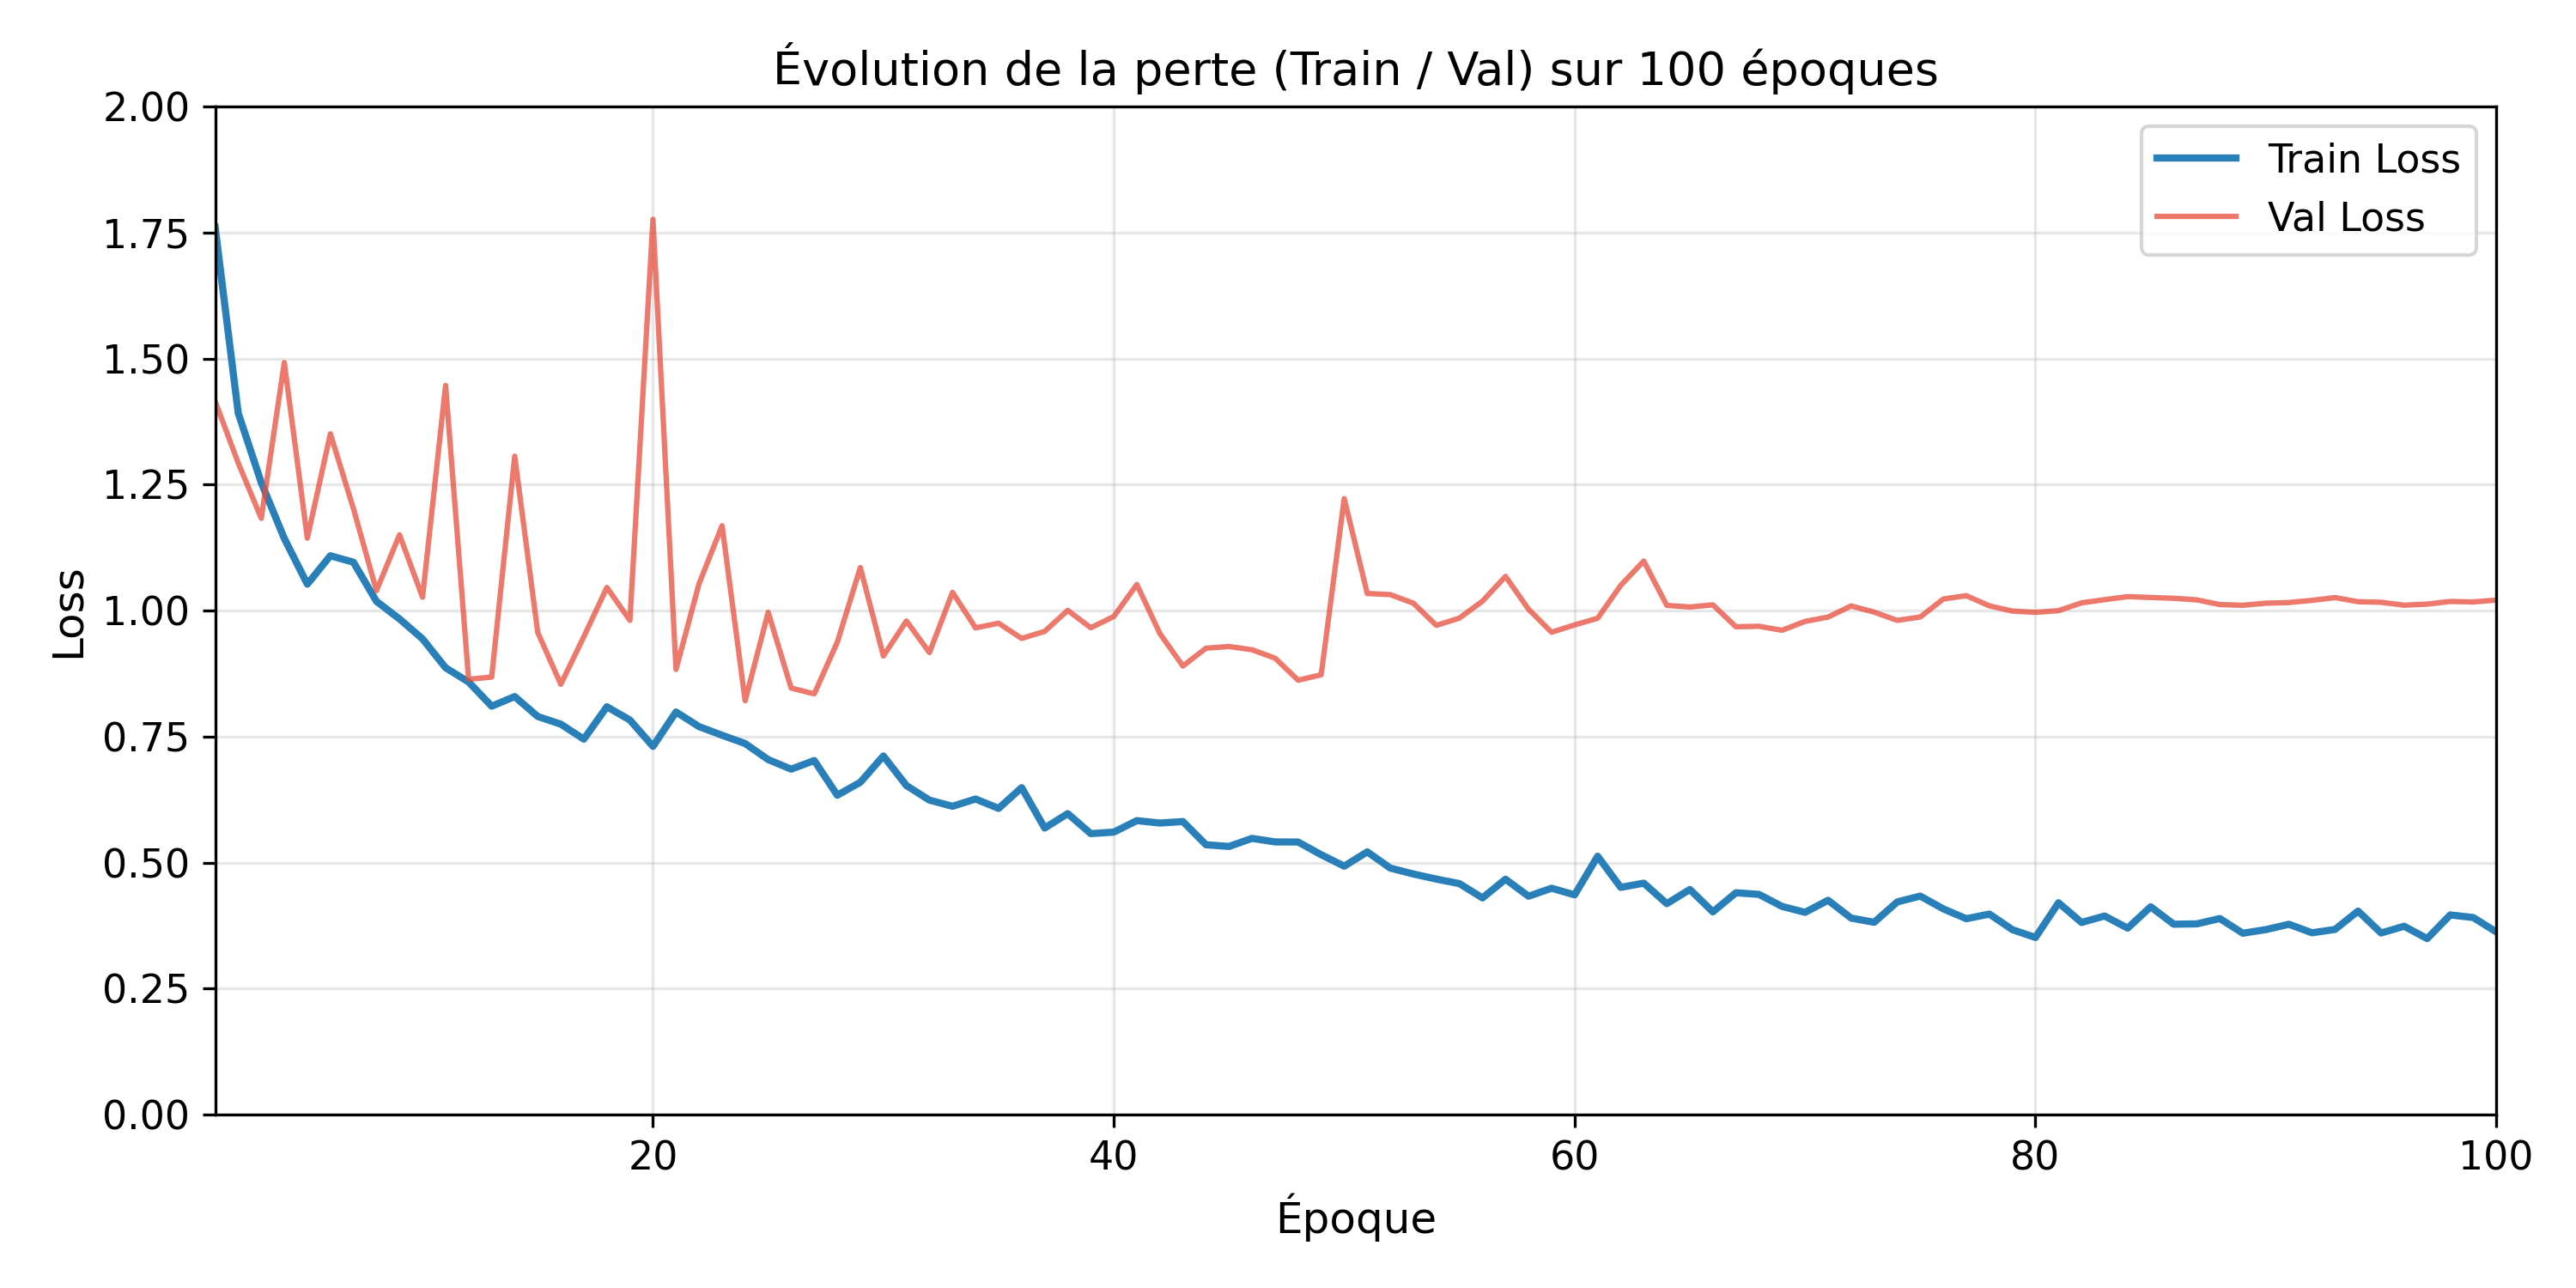
\includegraphics[width=0.85\textwidth]{loss_curve.png}
\caption{Évolution de la perte (train et validation) sur 100 époques.}
\label{fig:loss}
\end{figure}

La perte d'entraînement diminue de \textbf{1,76} à l'époque~1 à \textbf{0,36} à l'époque~100 ($-79\,\%$). La décroissance est rapide jusqu'à l'époque~20 (adaptation des couches finales au transfert learning), puis continue lentement. La perte de validation reste stable entre 0,85 et 1,06 à partir de l'époque~12, sans divergence, ce qui confirme l'absence de sur-apprentissage catastrophique sur les données de validation. Le meilleur checkpoint est sélectionné à l'époque~60, où le mAP@0.5 de validation atteint son maximum de \textbf{0,309}.

\subsection{Résultats quantitatifs --- Métriques d'évaluation}

Nous évaluons le modèle sur le \textbf{jeu de test} (10\,\% des données, $\sim$15 images isolées dès le début et jamais vues pendant l'entraînement) avec un seuil IoU de 0,5 et un seuil de confiance de 0,25. Le tableau~\ref{tab:metrics} résume les performances par classe.

\begin{table}[H]
\centering
\begin{tabularx}{\linewidth}{>{\raggedright\arraybackslash}X c c c c c c}
\toprule
\textbf{Classe} & \textbf{Labels} & \textbf{Precision} & \textbf{Recall} & \textbf{F1} & \textbf{mAP@0.5} \\
\midrule
\texttt{ferme}    & 6   & 0,333 & 0,167 & 0,222 & 0,194 \\
\texttt{immeuble} & 174 & 0,229 & 0,144 & 0,177 & 0,162 \\
\texttt{maison}   & 160 & 0,462 & 0,344 & 0,394 & 0,349 \\
\texttt{piscine}  & 31  & 0,684 & 0,419 & 0,520 & 0,586 \\
\texttt{usine}    & 8   & 0,000 & 0,000 & 0,000 & 0,000 \\
\texttt{villa}    & 3   & 0,000 & 0,000 & 0,000 & 0,000 \\
\midrule
\textbf{mAP@0.5 global} & & \multicolumn{4}{c}{\textbf{0,215}} \\
\bottomrule
\end{tabularx}
\caption{Precision, Recall, F1 et mAP@0.5 par classe sur le jeu de test (IoU $\geq$ 0,5, confiance $\geq$ 0,25).}
\label{tab:metrics}
\end{table}

Le modèle atteint un \textbf{mAP@0.5 de 0,215} sur le jeu de test. La classe \texttt{piscine} obtient les meilleurs résultats (F1~=~0,520, mAP~=~0,586), ce qui s'explique par sa couleur bleue caractéristique et visuellement distinctive dans l'imagerie satellite. La classe \texttt{maison}, malgré sa dominance dans le dataset, n'atteint qu'un F1 de 0,394, indiquant un surapprentissage partiel. Les classes \texttt{usine} et \texttt{villa} ne sont pas détectées (scores nuls), confirmant que leur très faible représentation ($<$70 et 17 annotations respectivement) est insuffisante pour que le modèle apprenne des caractéristiques généralisables, même avec sur-échantillonnage.

La figure~\ref{fig:pr_class} illustre ces métriques sous forme de diagramme en barres.

\begin{figure}[H]
\centering
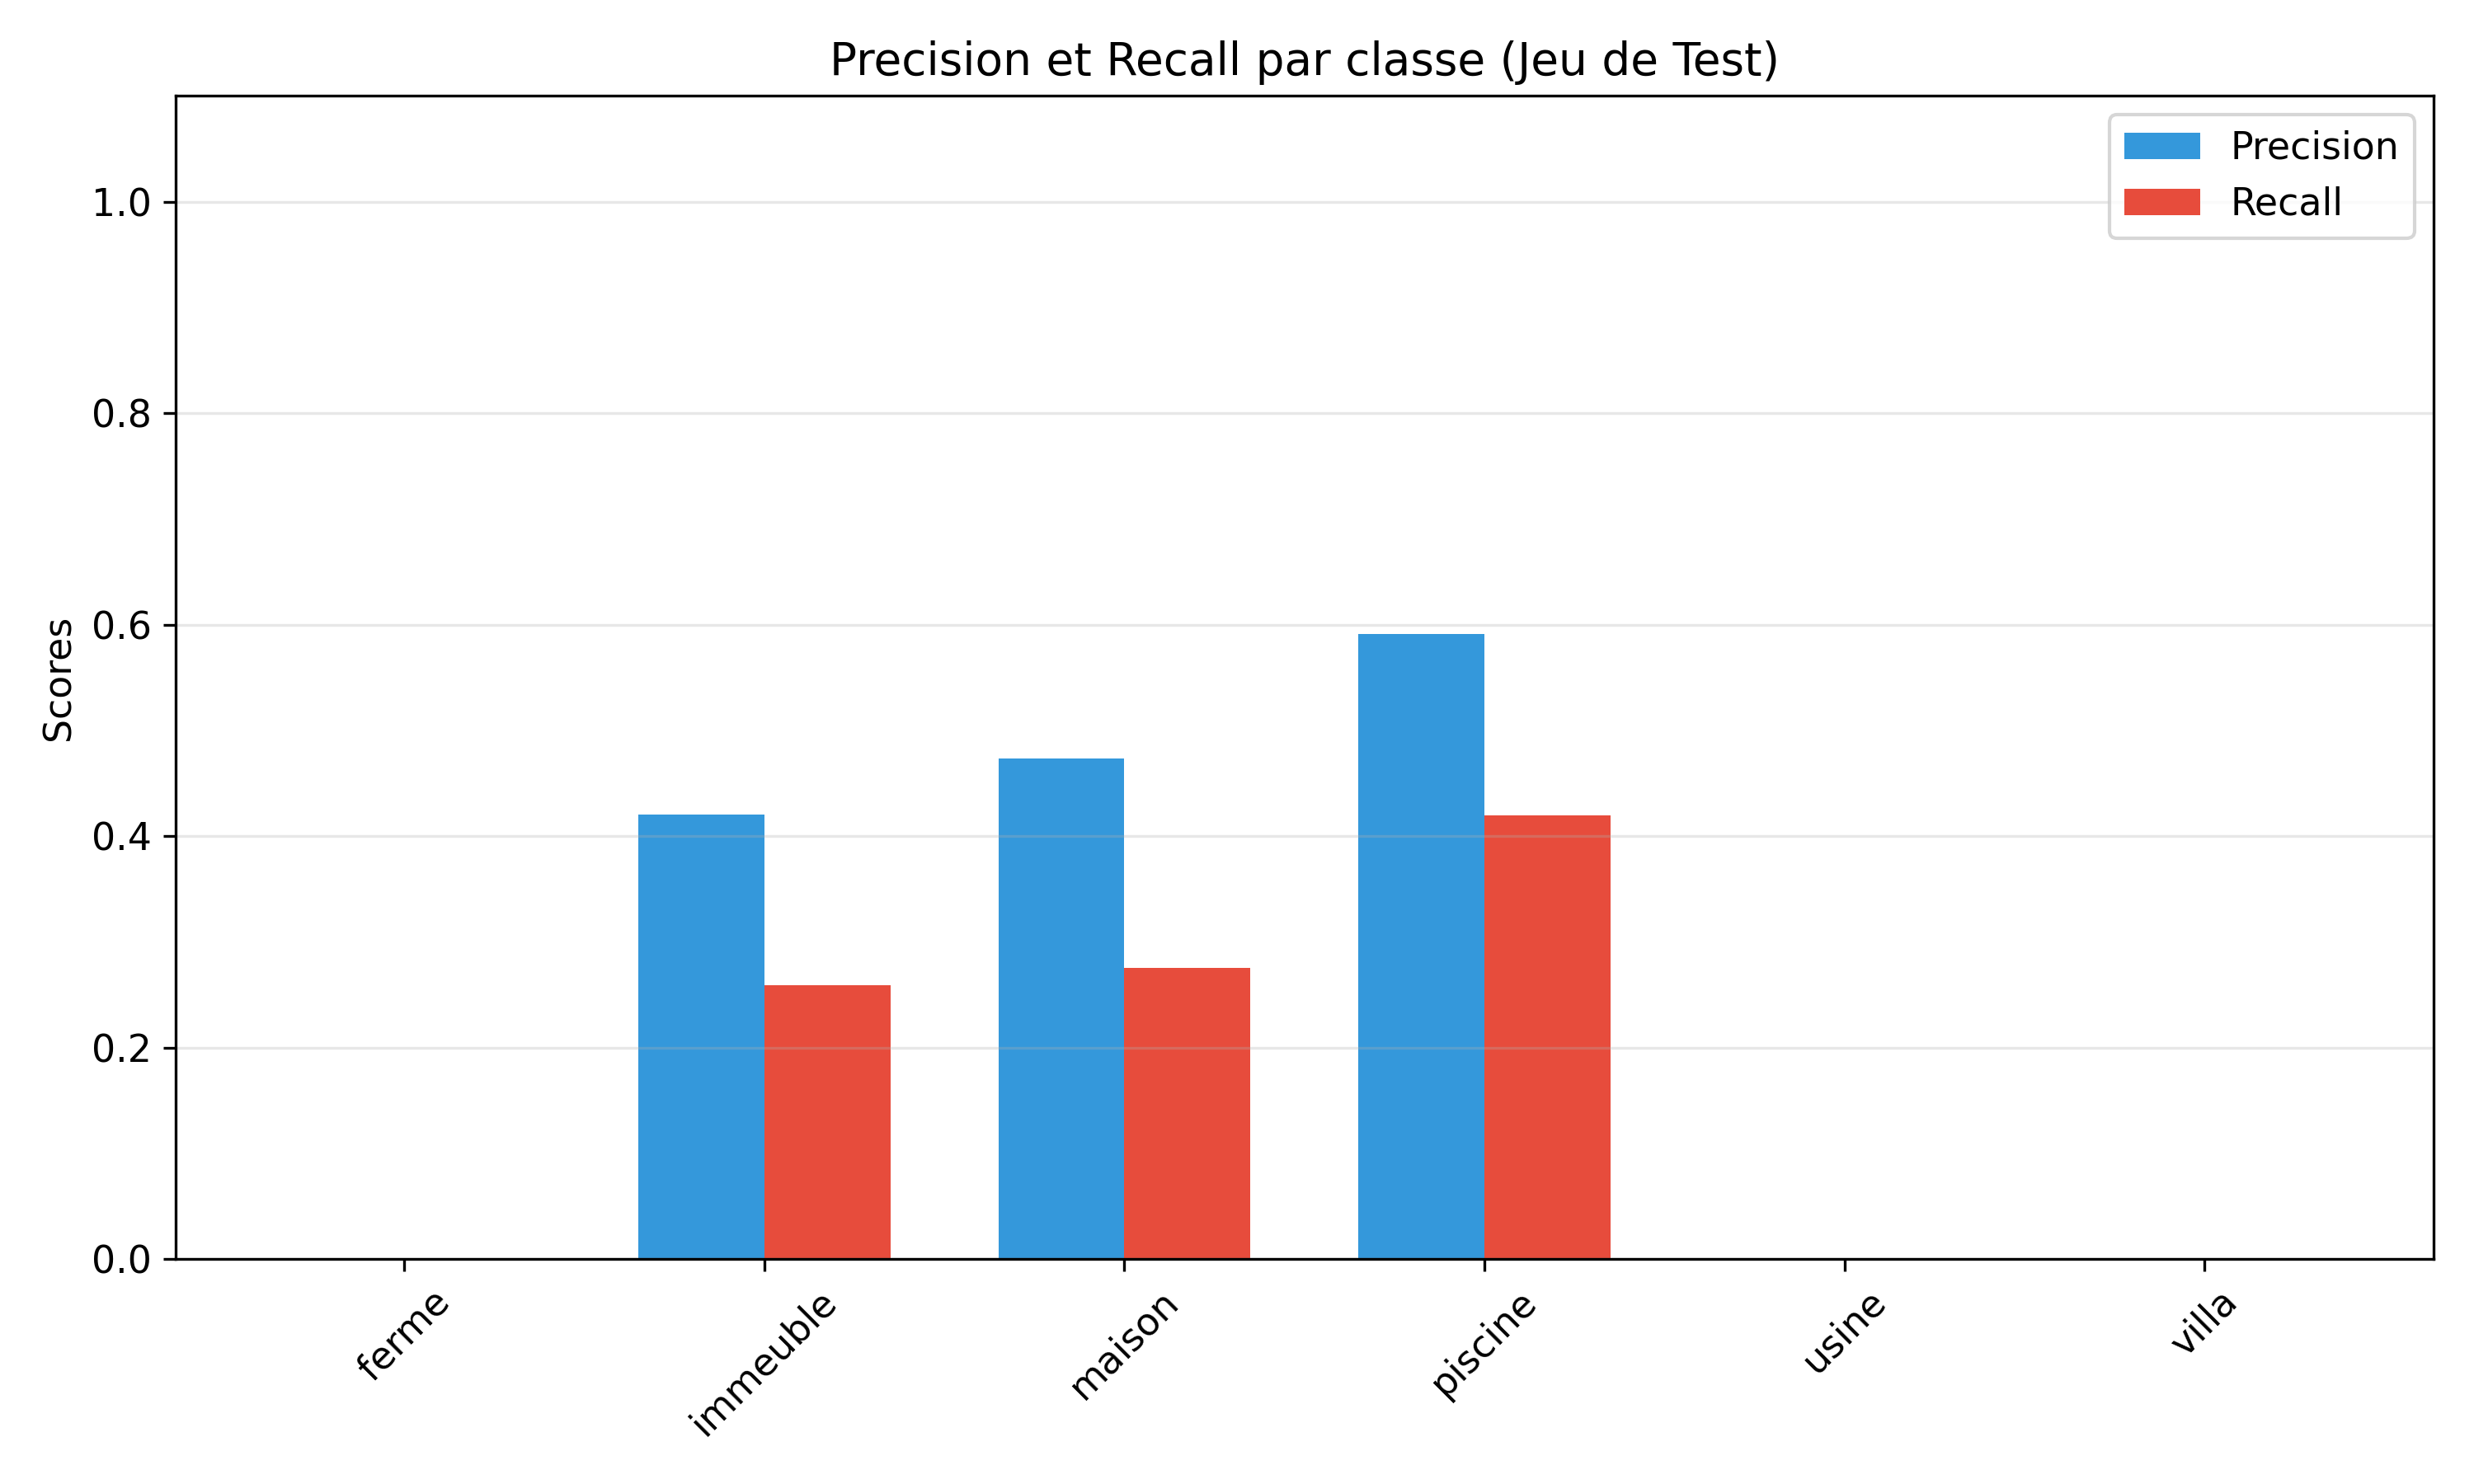
\includegraphics[width=0.85\textwidth]{precision_recall_per_class.png}
\caption{Precision et Recall par classe.}
\label{fig:pr_class}
\end{figure}

\subsection{Matrice de confusion}

La matrice de confusion (figure~\ref{fig:confusion}) met en évidence les confusions entre classes.

\begin{figure}[H]
\centering
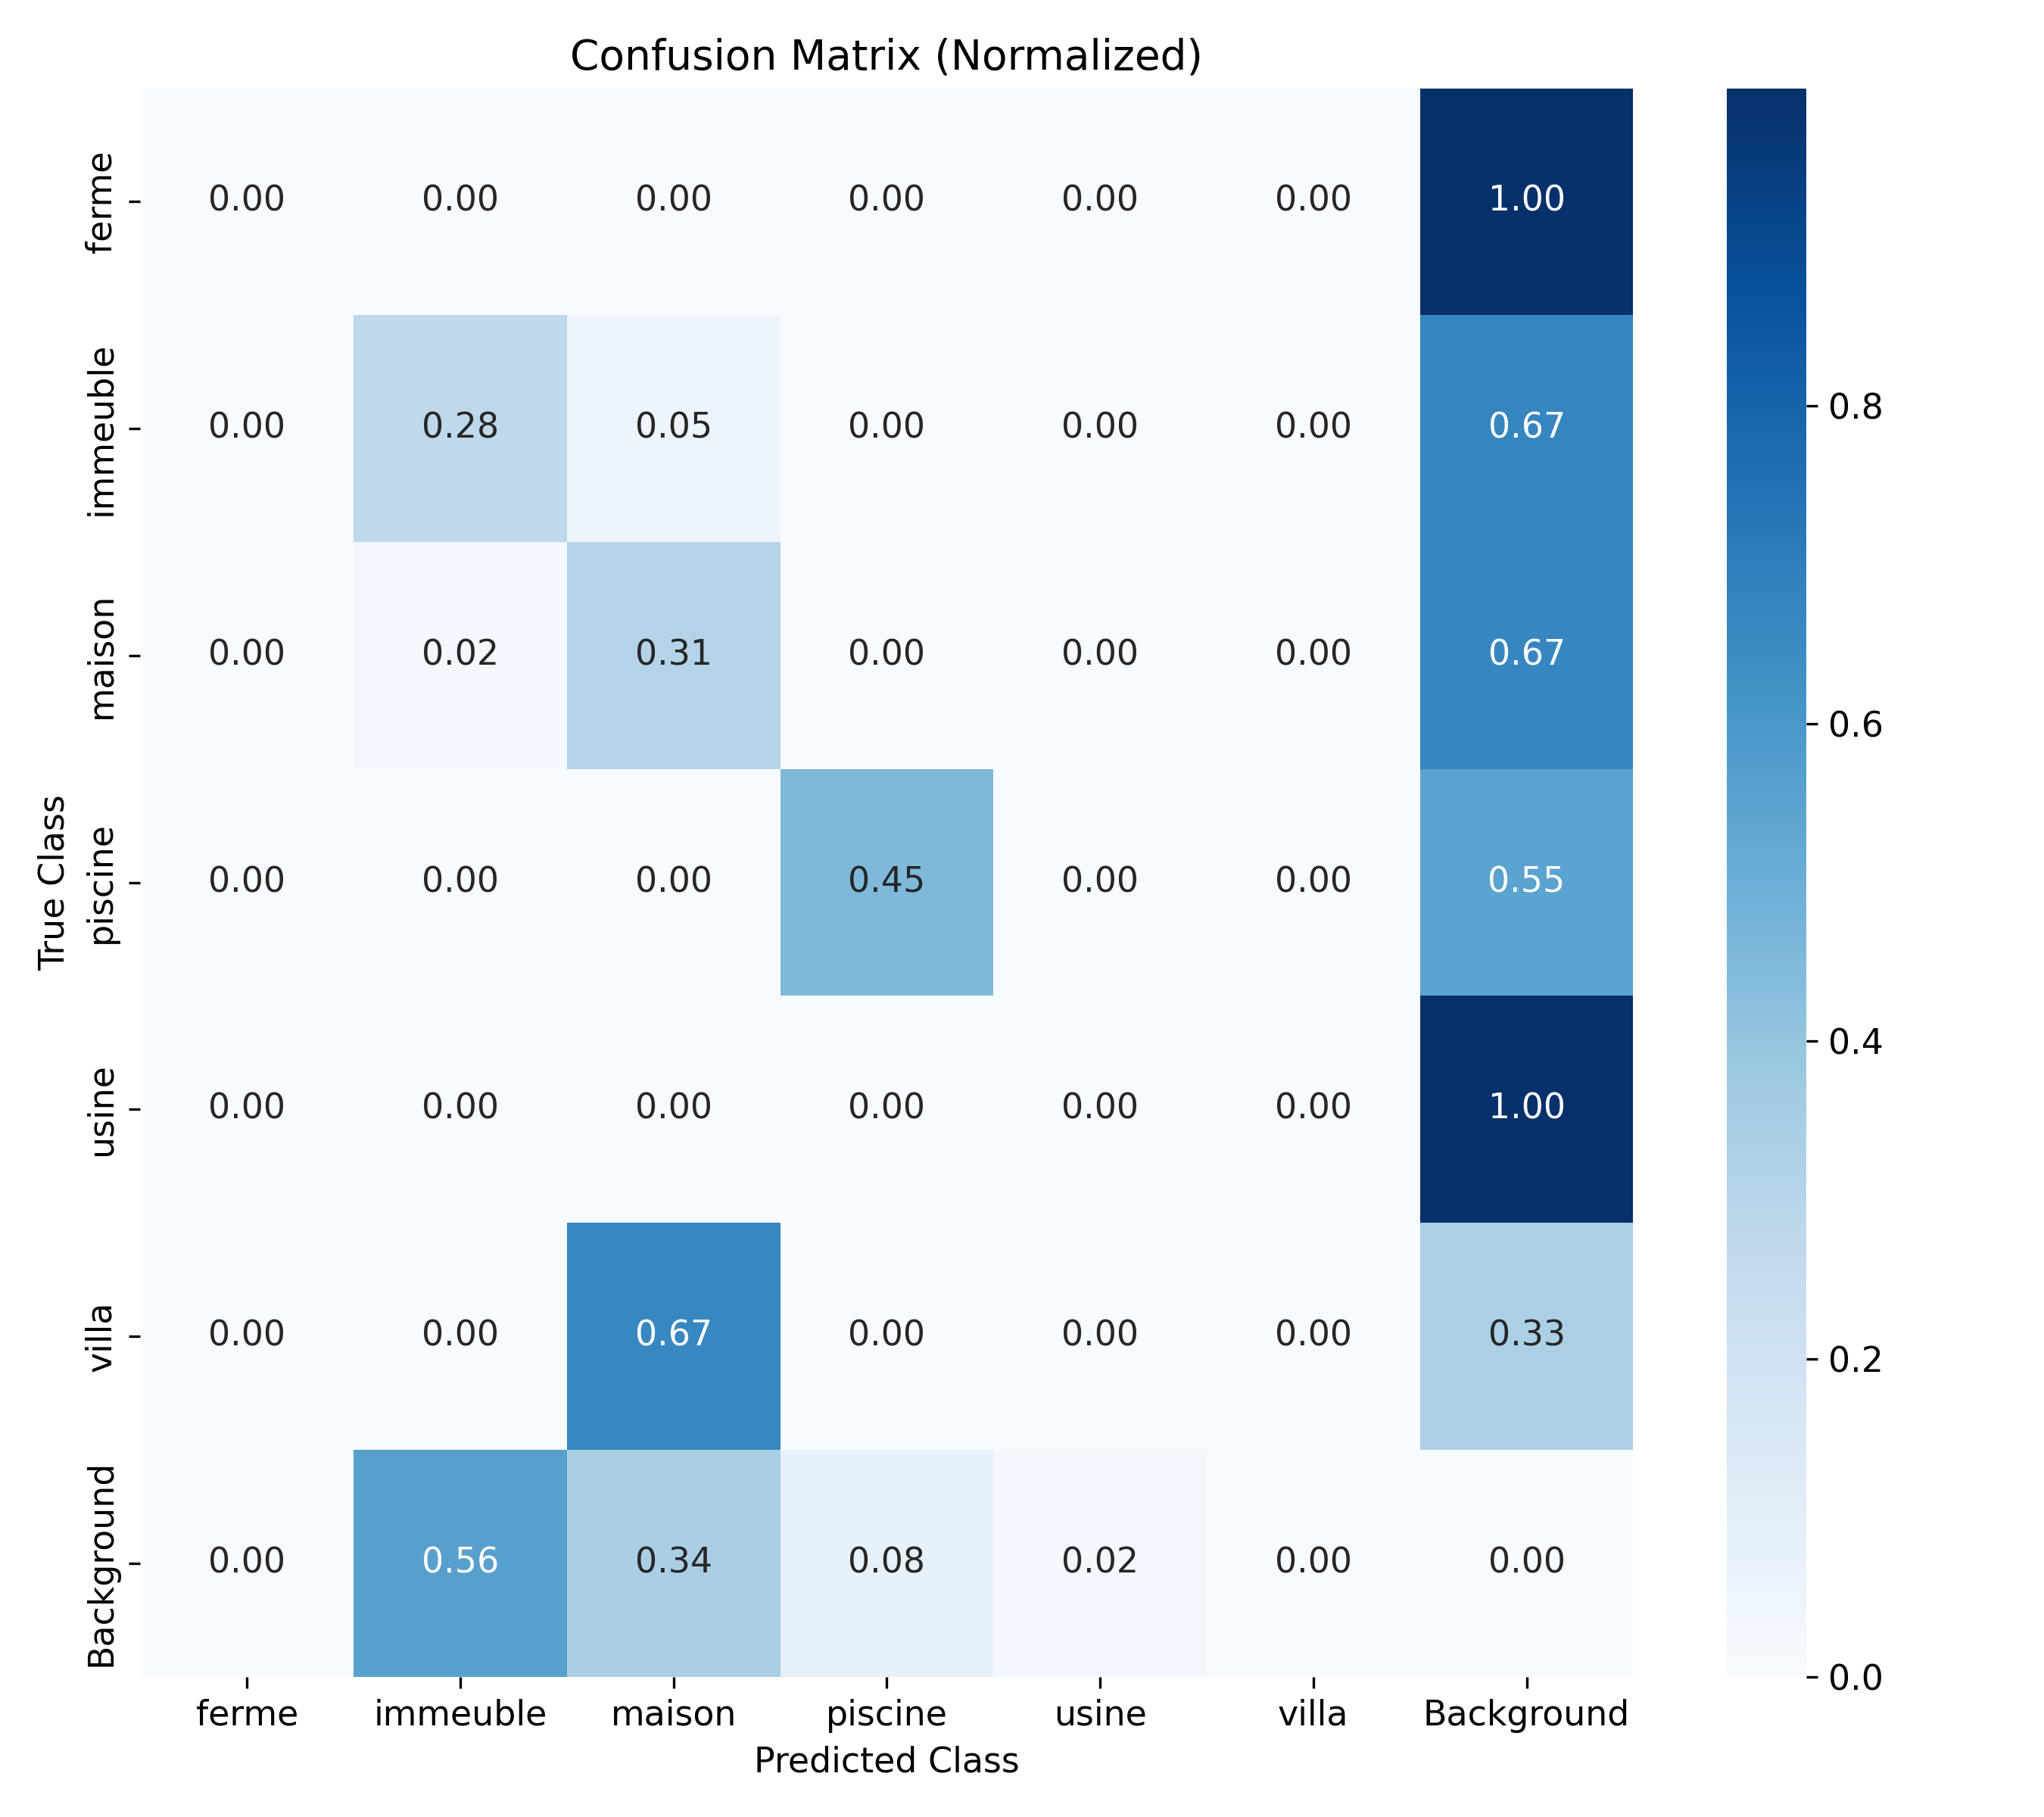
\includegraphics[width=0.75\textwidth]{confusion_matrix.png}
\caption{Matrice de confusion normalisée (IoU $\geq$ 0,5).}
\label{fig:confusion}
\end{figure}

La matrice de confusion confirme que les confusions les plus fréquentes se produisent entre classes visuellement proches. En particulier, les \texttt{immeubles} sont souvent confondus avec les \texttt{maisons}, ce qui s'explique par des empreintes au sol parfois similaires en vue satellite. Les \texttt{piscines} génèrent un nombre élevé de faux positifs, probablement dû à la détection de surfaces bleues (bâches, ombres) qui ne sont pas des piscines. Les classes minoritaires (\texttt{usine}, \texttt{villa}) montrent une faible couverture en recall en raison de leur sous-représentation dans le jeu d'entraînement.

\subsection{Résultats qualitatifs --- Inférence}

L'inférence est réalisée dans le notebook \texttt{Plots\_for\_report.ipynb} avec les paramètres suivants :
\begin{itemize}
    \item Seuil de confiance : \texttt{conf\_thres = 0.25}
    \item Seuil IoU (NMS) : \texttt{iou\_thres = 0.45}
\end{itemize}

Le processus d'inférence comprend :
\begin{enumerate}
    \item \textbf{Redimensionnement} simple à $640 \times 640$ (étirement, \texttt{PIL.Image.resize}).
    \item \textbf{Propagation avant} dans le modèle en mode \texttt{eval()}.
    \item \textbf{Non-Maximum Suppression} (NMS) pour filtrer les détections redondantes.
    \item \textbf{Remise à l'échelle} des \emph{bounding boxes} vers les coordonnées de l'image originale.
    \item \textbf{Visualisation} : dessin des boîtes avec étiquettes (\texttt{classe + confiance}) sur l'image.
\end{enumerate}

\subsubsection{Cas réussis}

La figure~\ref{fig:success} présente trois exemples de détections réussies par le modèle. Les \emph{bounding boxes} vertes représentent la vérité terrain et les boîtes colorées les prédictions du modèle.

\begin{figure}[H]
\centering
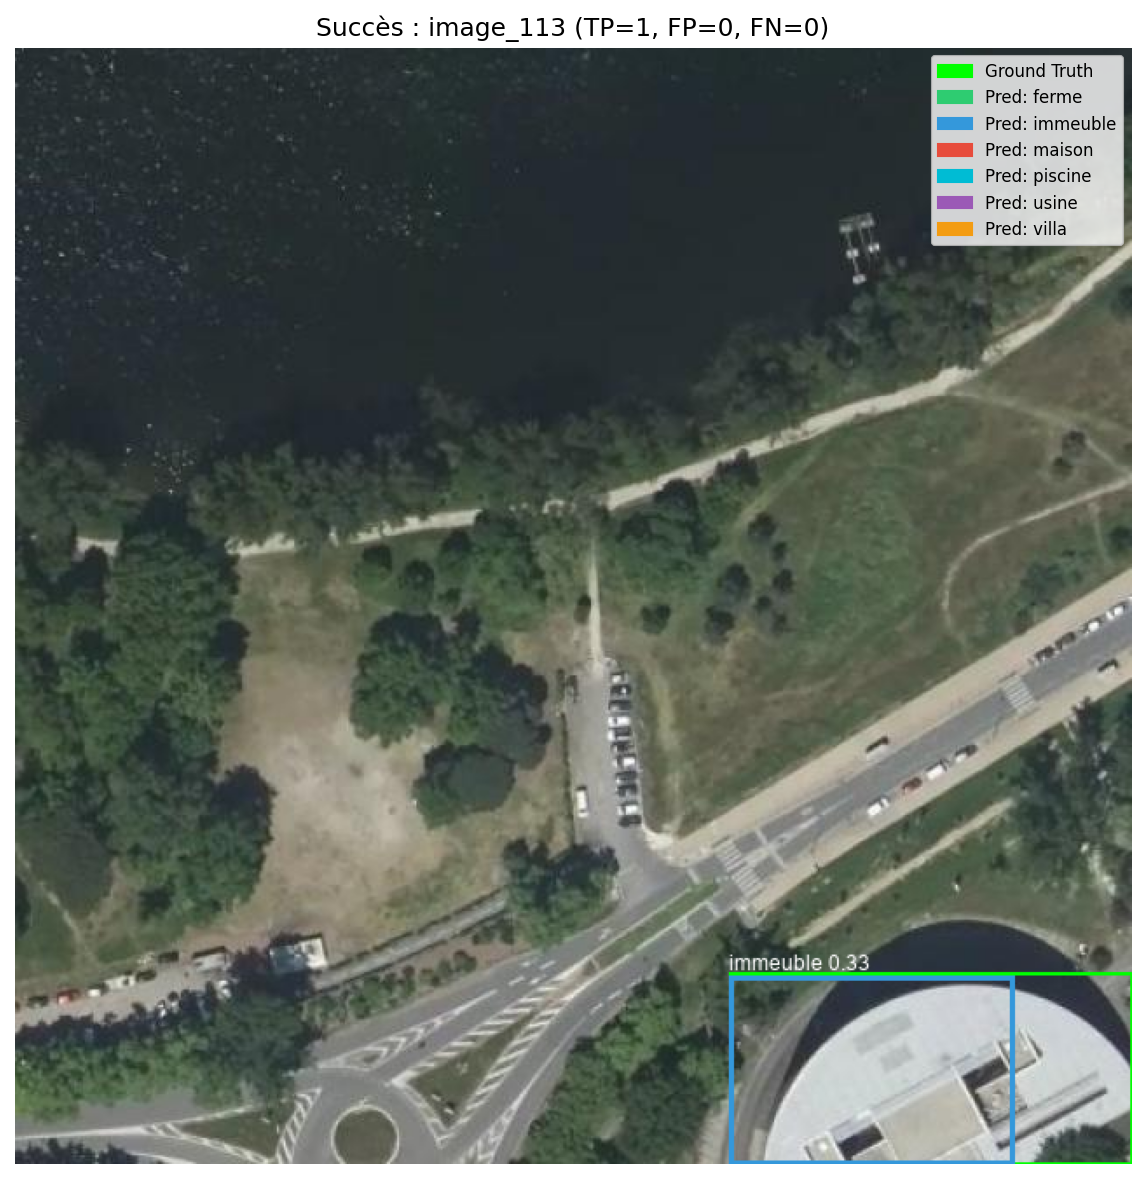
\includegraphics[width=0.32\textwidth]{prediction_success_1.png}
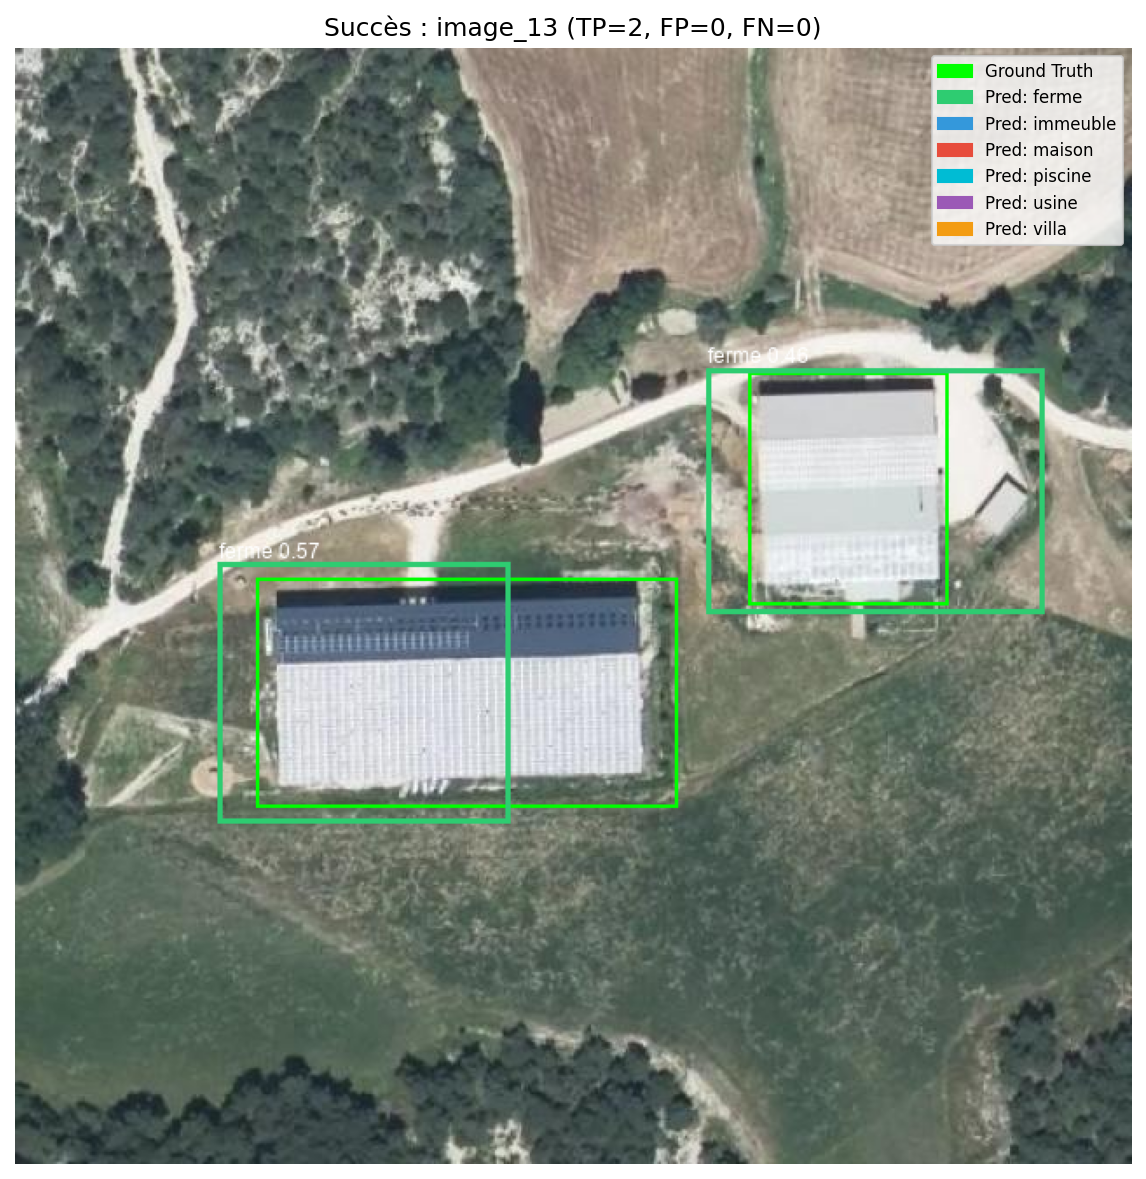
\includegraphics[width=0.32\textwidth]{prediction_success_2.png}
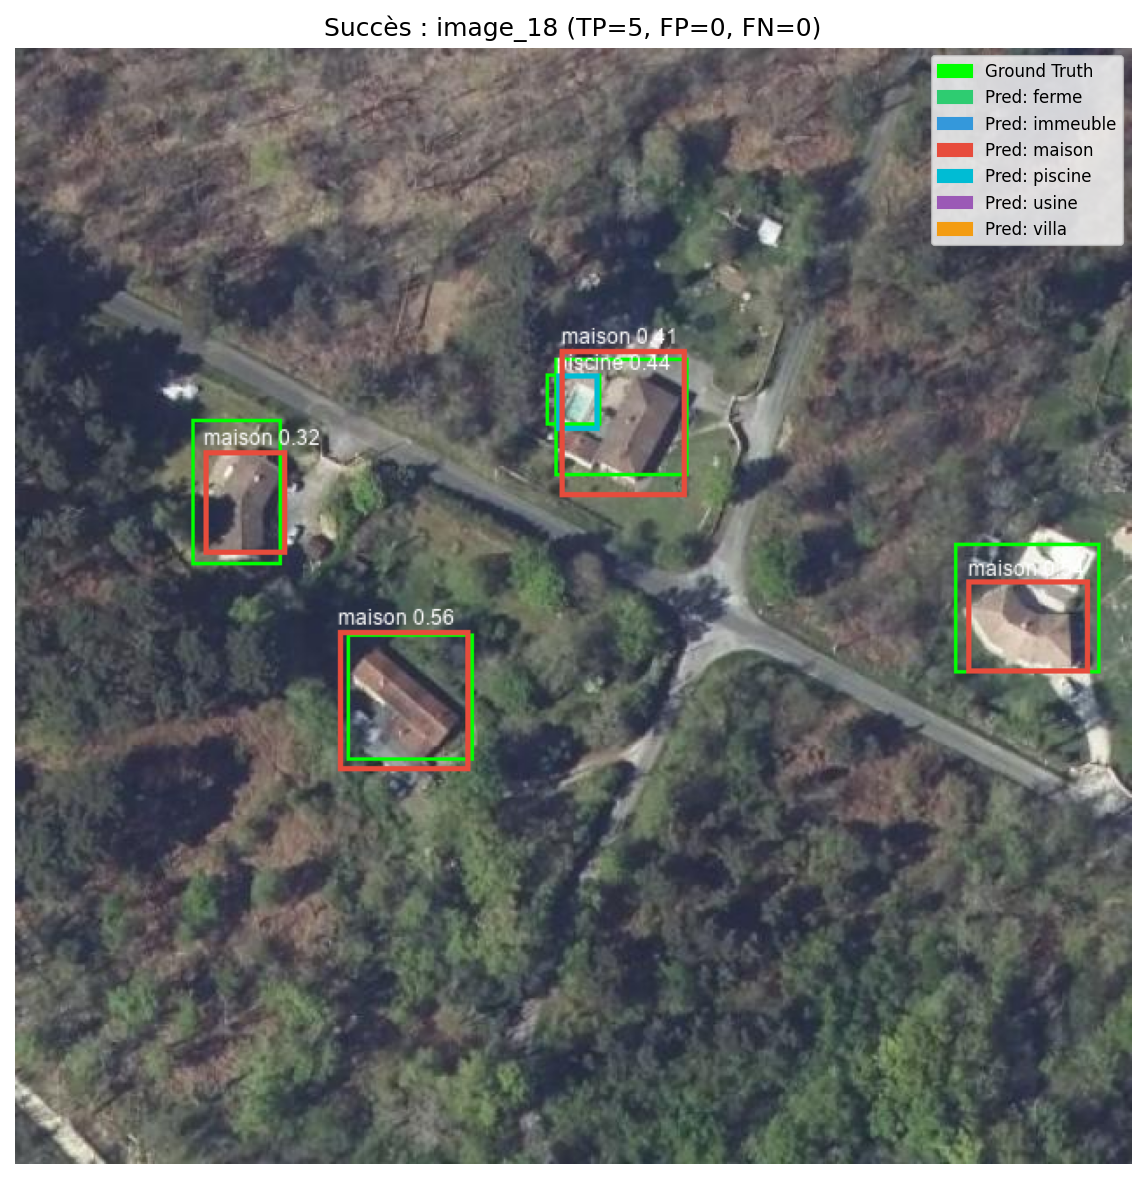
\includegraphics[width=0.32\textwidth]{prediction_success_3.png}
\caption{Exemples de détections réussies (vert = GT, couleur = prédiction).}
\label{fig:success}
\end{figure}

Le modèle détecte correctement :
\begin{itemize}
    \item Les \textbf{maisons} en zone résidentielle dense, classe la plus représentée dans le jeu de données.
    \item Les \textbf{immeubles} de grande taille, facilement distinguables par leur empreinte au sol.
    \item Les \textbf{piscines}, dont la couleur bleue caractéristique les rend saillantes dans l'imagerie satellite.
\end{itemize}

\subsubsection{Erreurs courantes}

La figure~\ref{fig:failures} montre trois exemples où le modèle commet des erreurs significatives.

\begin{figure}[H]
\centering
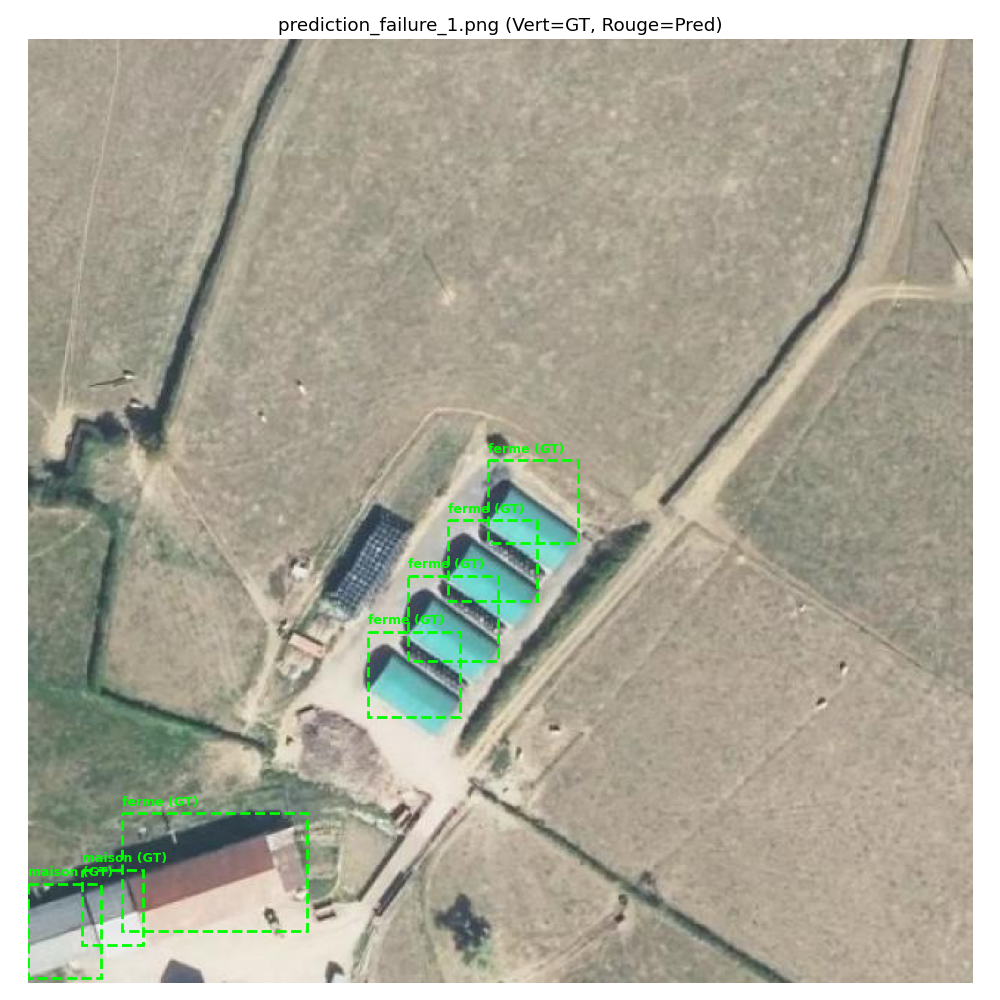
\includegraphics[width=0.32\textwidth]{prediction_failure_1.png}
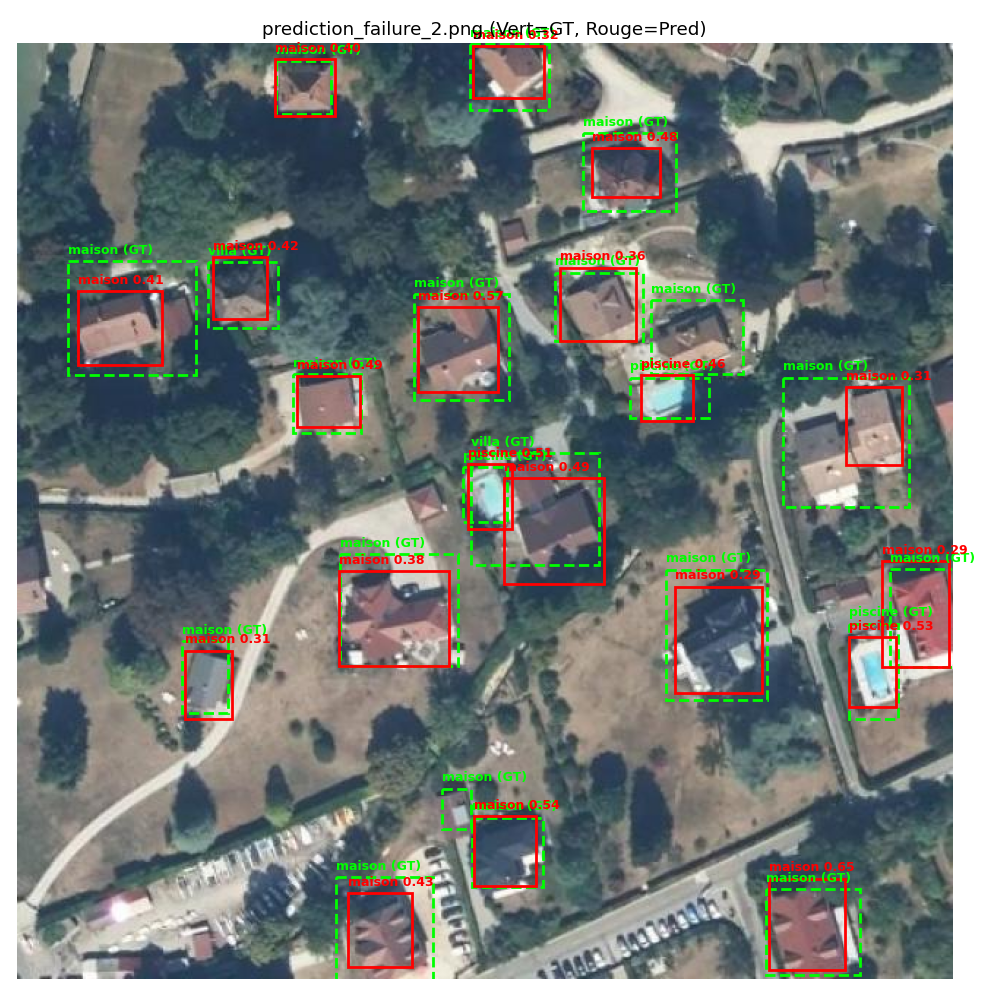
\includegraphics[width=0.32\textwidth]{prediction_failure_2.png}
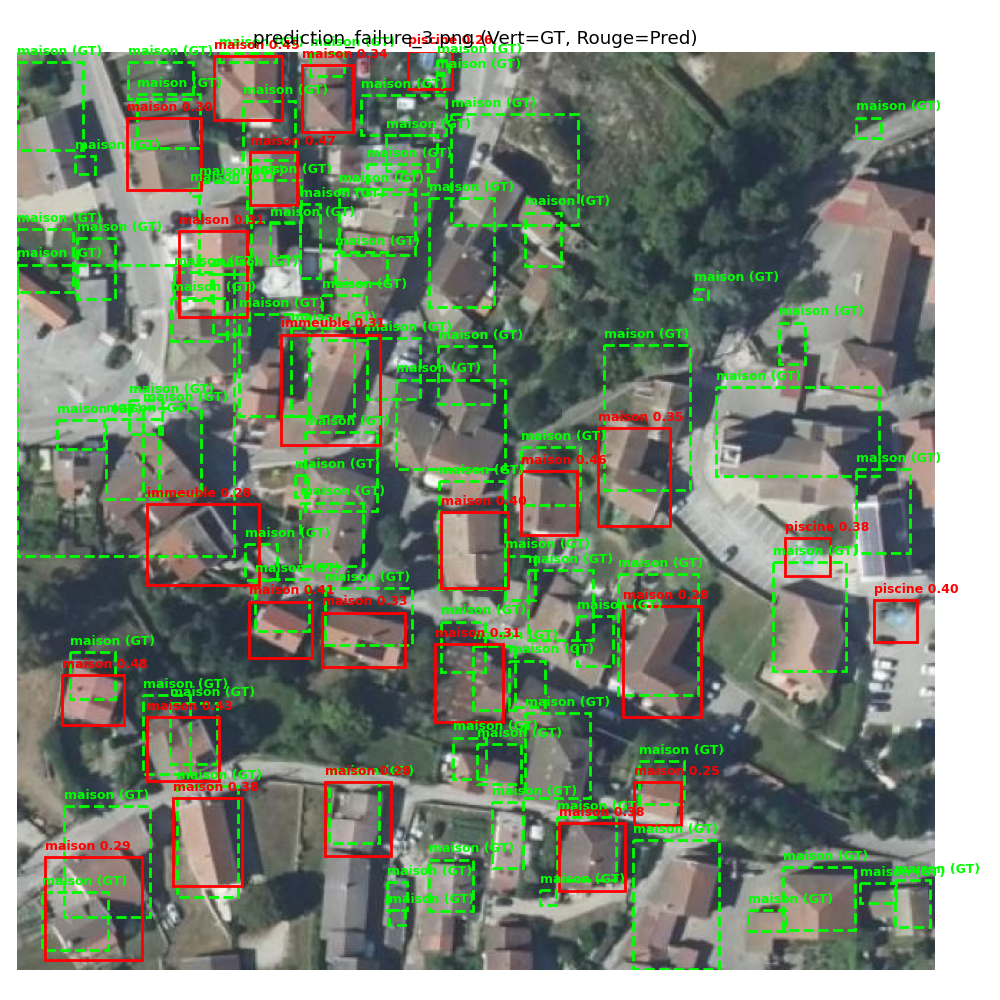
\includegraphics[width=0.32\textwidth]{prediction_failure_3.png}
\caption{Exemples d'erreurs de détection (vert = GT, couleur = prédiction).}
\label{fig:failures}
\end{figure}

Les difficultés principales observées incluent :
\begin{itemize}
    \item \textbf{Confusion maison/villa} : ces deux classes sont visuellement très proches sur images satellites.
    \item \textbf{Fermes vs usines} : les grands bâtiments agricoles et industriels ont des empreintes au sol similaires.
    \item \textbf{Bruit d'annotation} : les annotations automatiques via OSM peuvent contenir des erreurs (tags manquants ou incorrects, décalage géographique).
    \item \textbf{Taille du jeu de données} : avec 144 images et 6 classes, le nombre d'exemples par classe est limité, ce qui peut conduire à un sur-apprentissage ou à une mauvaise généralisation.
\end{itemize}

% =====================================================================
\section{Discussion et perspectives}\label{sec:discussion}
% =====================================================================

\subsection{Bilan}

Ce projet démontre la faisabilité d'un pipeline complet de détection d'objets sur imagerie satellitaire, allant de la collecte automatisée des données à l'inférence. Les points forts sont :

\begin{itemize}
    \item Un \textbf{pipeline de collecte automatisé} combinant Mapbox (images) et OSM (annotations), reproductible et extensible à de nouvelles zones géographiques.
    \item L'utilisation du \textbf{transfer learning} avec YOLOv5n pré-entraîné sur COCO, permettant une convergence rapide malgré un jeu de données restreint.
    \item Une \textbf{architecture légère} (1,9\,M paramètres) adaptée à la taille du jeu de données.
\end{itemize}

\subsection{Limites}

\begin{itemize}
    \item \textbf{Taille du jeu de données} : 144 images est en deçà de l'idéal pour 6 classes. L'augmentation de données (mosaïque, flip, HSV) compense partiellement ce déficit.
    \item \textbf{Qualité des annotations} : les annotations automatiques OSM ne sont pas toujours précises. Un passage par Roboflow a permis une correction manuelle partielle.
    \item \textbf{Taille critique du jeu de test} : avec un split 80/10/10, le jeu de test ne contient qu'environ 15~images. Les métriques sont donc instables et peu représentatives --- une variation de 1 TP peut changer le F1 de plusieurs points de pourcentage.
    \item \textbf{Surapprentissage} : le modèle mémorise une partie des données d'entraînement. La loss décroît régulièrement mais les performances sur données inconnues restent limitées (mAP~0,215), signe d'un dataset insuffisant pour 6~classes.
    \item \textbf{Déséquilibre des classes} : avec 1\,245 annotations pour \texttt{maison} contre seulement 17 pour \texttt{villa} et 69 pour \texttt{usine}, les classes rares ne sont pas détectées malgré le sur-échantillonnage.
\end{itemize}

\subsection{Bilan comparatif des approches}

Deux configurations d'entraînement ont été évaluées sur le \textbf{même jeu de test} (15~images, jamais vues) afin de mesurer l'impact des modifications apportées.

\begin{table}[H]
\centering
\begin{tabularx}{\linewidth}{>{\raggedright\arraybackslash}X c c}
\toprule
\textbf{Configuration} & \textbf{mAP@0.5 (test)} & \textbf{Classes détectées} \\
\midrule
Baseline : 50~ép., BCE, shuffle & 0,070 & maison, piscine \\
Amélioré : 100~ép., FL $\gamma$=1,5, sampler, flip & \textbf{0,215} & ferme, immeuble, maison, piscine \\
\bottomrule
\end{tabularx}
\caption{Comparaison des deux configurations sur le jeu de test (IoU $\geq$ 0,5).}
\label{tab:compare}
\end{table}

L'approche améliorée multiplie le mAP par 3 ($\times$3,1) par rapport à la baseline. Les modifications apportées --- Focal Loss~[8], WeightedRandomSampler et augmentation géométrique --- ont permis au modèle de détecter deux classes supplémentaires (\texttt{ferme} et \textbf{immeuble}) sur le jeu de test. Cependant, \texttt{usine} et \texttt{villa} restent indétectables (scores nuls), leurs trop faibles représentations dans le dataset (69 et 17 annotations) étant insuffisantes pour une généralisation, même avec sur-échantillonnage $\times$4.

\noindent\textbf{Note sur l'évaluation.} Une évaluation erronée sur l'ensemble des 144~images (entraînement inclus) avait initialement donné un mAP apparent de 0,621, masquant le surapprentissage. Les chiffres ci-dessus (0,070 et 0,215) sont calculés \emph{exclusivement} sur les 15~images de test, jamais exposées à l'entraînement.

\subsection{Autres pistes non implémentées}

\begin{itemize}
    \item \textbf{Augmenter le volume de données} : le pipeline Mapbox/OSM est extensible à d'autres coordonnées ou pays pour atteindre 400+ images.
    \item \textbf{Modèle plus grand} : YOLOv5s (7~M params) ou YOLOv8n avec un dataset élargi.
    \item \textbf{Recalcul des anchors} : \texttt{autoanchor} pourrait optimiser les anchors aux tailles des bâtiments satellitaires.
    \item \textbf{Segmentation d'instance} : YOLOv5-seg permettrait des contours plus précis que les bounding boxes.
\end{itemize}

% =====================================================================
\section{Conclusion}
% =====================================================================

Ce projet a permis de développer un système complet de détection de bâtiments sur imagerie satellitaire, couvrant la collecte automatisée de données, l'annotation, l'entraînement d'un modèle de détection d'objets par transfert d'apprentissage, et l'inférence.

L'architecture YOLOv5 Nano, entraînée sur 100 époques avec Focal Loss ($\gamma$=1,5), sur-échantillonnage des classes rares et augmentation géométrique, atteint un \textbf{mAP@0.5 de 0,215} sur le jeu de test (15 images non vues). Ce résultat reflète la difficulté intrinsèque du problème : 144 images pour 6 classes avec un déséquilibre extrême (17 annotations pour \texttt{villa} contre 1\,245 pour \texttt{maison}). Les améliorations apportées ont permis de tripler le mAP par rapport à la baseline (0,070), avec 4 classes détectées sur 6. Le pipeline développé --- de la collecte Mapbox/OSM à l'inférence --- est entièrement reproductible et extensible à de nouvelles zones géographiques, constituant une base solide pour de futures améliorations.

% =====================================================================
\section*{Références}
% =====================================================================

\begin{enumerate}
    \item Redmon, J., Divvala, S., Girshick, R., \& Farhadi, A. (2016). \textit{You Only Look Once: Unified, Real-Time Object Detection}. CVPR 2016.
    \item Jocher, G. (2020). \textit{YOLOv5 by Ultralytics}. \url{https://github.com/ultralytics/yolov5}
    \item Boeing, G. (2017). \textit{OSMnx: New Methods for Acquiring, Constructing, Analyzing, and Visualizing Complex Street Networks}. Computers, Environment and Urban Systems, 65, 126--139.
    \item Mapbox. \textit{Static Images API}. \url{https://docs.mapbox.com/api/maps/static-images/}
    \item Roboflow. \textit{Computer Vision Platform}. \url{https://roboflow.com}
    \item Lin, T.-Y. et al. (2014). \textit{Microsoft COCO: Common Objects in Context}. ECCV 2014.
    \item Zheng, Z. et al. (2020). \textit{Distance-IoU Loss: Faster and Better Learning for Bounding Box Regression}. AAAI 2020.
    \item Lin, T.-Y. et al. (2017). \textit{Focal Loss for Dense Object Detection}. ICCV 2017 (RetinaNet).
\end{enumerate}

\end{document}
